\documentclass[a4,12pt,showpacs,preprintnumbers,amsmath,amssymb]{revtex4}
\usepackage[utf8]{inputenc}
\usepackage{amsmath,amsfonts,amssymb}
\usepackage[english]{babel}
\usepackage{graphicx}
\usepackage{caption}
\captionsetup{justification=raggedright,singlelinecheck=false}
\usepackage{array}
\usepackage{textcomp}
\usepackage{color}
\usepackage{url}
\usepackage{makecell}
\newcommand{\MCM}[1]{\noindent{\marginpar{\bf \tiny MCM} \bf  #1 }}
\newcommand{\wes}[1]{\noindent{\marginpar{\bf \tiny Wesley} \textcolor{blue}{  #1 }}}
\linespread{1.4}               % extra vertical space inserted before
\setlength{\parskip}{3.0ex}    % the paragraph
%...End lines and paragraphs

\usepackage{layout}        %with the command layot print the format of the page
\usepackage{color}
\usepackage{graphicx}% Include figure files
\usepackage{dcolumn}% Align table columns on decimal point
\usepackage{bm}% bold math
\usepackage[colorlinks]{hyperref}




\newcolumntype{x}[1]{>{\centering\arraybackslash}p{#1}}
\usepackage{tikz}
\newcommand\diag[4]{%
  \multicolumn{1}{p{#2}|}{\hskip-\tabcolsep
  $\vcenter{\begin{tikzpicture}[baseline=0,anchor=south west,inner sep=#1]
  \path[use as bounding box] (0,0) rectangle (#2+2\tabcolsep,\baselineskip);
  \node[minimum width={#2+2\tabcolsep-\pgflinewidth},
        minimum  height=\baselineskip+\extrarowheight-\pgflinewidth] (box) {};
  \draw[line cap=round] (box.north west) -- (box.south east);
  \node[anchor=south west] at (box.south west) {#3};
  \node[anchor=north east] at (box.north east) {#4};
 \end{tikzpicture}}$\hskip-\tabcolsep}}
\newcommand{\angstrom}{\text{\normalfont\AA}}

\begin{document}

% Title Page
\title{He--vacancy interactions in Vanadium and Tantalum}
\author{Wesley Unn-Toc, Mihai-Cosmin Marinica, Thomas Jourdan}
\affiliation{DEN-Service de Recherches de M\'etallurgie Physique, CEA, Université Paris-Saclay, F-91191, Gif-sur-Yvette, France}
\date{}

\begin{abstract}
In this paper we investigate the energy landscape of vacancy clusters in the presence of Heliun in two materials, 
Vanadium and Tantalum. 
In order to address the relative stability of small vacancy-Helium clusters as well as the basic migration 
mechanisms we have used Density Functional Theory. 
The results of calculations are systematized in simple laws that can be easily used subsequently 
in multi-scale techniques including kinetic Monte Carlo simulations and cluster dynamics or dislocation dynamics studies.
\end{abstract}
\pacs{61.72.Jj, 61.72.Bb, 61.80.Az, 61.82.Bg, 75.40.Mg}


 \maketitle
 
\section{Introduction}

The main materials of interest for  fission and fusion application are the body centered cubic (bcc) metals, 
such as transition metals. 
%
Irradiation of bcc transition metals, leads to a large number of point defects in the form of self-interstitial 
atoms and vacancies. The interactions and migrations of defects as well as theirs absorption on sinks, 
like dislocation and grain boundaries, can influence microstructural transformations in material 
which can affect various properties of the metals. 
%
Experimental and theoretical studies \cite{Zinkle2013} have shown that the body centered cubic lattice demonstrates 
improved radiation resistance compared to the close-packed face centered cubic lattice due to reduced amount of 
vacancy and interstitial defect clustering that occurs directly within displacement cascades as well as 
higher stacking fault energy.
In this paper we will focus on the vacancy clusters and its interactions with Helium atoms in two materials promising 
for future fusion systems, V and Ta.   


%About Va and Ta 
V and its alloys are promising candidates as blanket for fusion reactor thanks 
to their mechanical properties at high temperature and low activation \cite{Muroga2000, Kurtz2004}.
V alloys demonstrate a good combination of strength, ductility and radiation resistance~\cite{Zinkle1998,Muroga2000}.  
%
Ta is known for its high toughness, high-sputtering threshold energy, easy fabricability and 
low activation properties which make it a candidate for target material for spallation sources or 
even first wall material in fusion reactors~\cite{Gold1979, Kirk1981}. As such, study of defects in those two materials,  
V and Ta serve as the basic foundation for future research regarding structural materials in the fusion industry.


%About defetcs ... 
Under irradiation, the structural materials are subject to damages such as swelling \cite{Dai2012141}, 
embrittlement \cite{MATSUI1992} and blistering \cite{KALETTA1978} 
triggered, enhanced  or suppressed \cite{FEDEROV1996} by He resulting of (\textit{n, $\alpha$}) transmutation reactions. 
He atoms are usually trapped at grain boundaries, dislocations or void clusters \cite{Bhattacharyya1997,HEERSCHAP1973}.
The early stages of formation of He bubbles in metals are difficult to be treated in experiments due to the spatial resolutions.  
\textit{Ab inito} calculations , based on Density Functional Theory (DFT), 
are powerful tools to investigate the processes taking place at the beginning of 
nucleation of such objects. The DFT calculations provide quantitative insight into 
the nature of clusters containing a small number of defects.
%
\wes{Only in recent years, such studies on V began and there is few literature concerning Ta. 
Hua et al.\cite{Hua20151} went to the conclusion that alloying V with Ti enhances migration energy of He and diminishes He-vacancy 
binding energy.
Zhang et al.\cite{Zhang201190} studied interaction of He with monovacancy and SIA in pure V and V alloys. 
They shown V alloy increases the cost of formation and migration of He compared to pure V solid. 
The same group investigated stability of small He-vacancy clusters and migration of monovacancy. 
They found that interstitial He clusters are weakly bound and need vacancy to be stable \cite{Zhang20111}.
The formation of He and vacancy at grain boundary in V has been investigated in Ref.\cite{Zhang2015121}.
He-He and He-metal interactions have been studied in various bcc transition metals \cite{Zhang2015}.
Energetics of interstitials He in several metals of $V$ group and $VI$ group have been detailed in Ref.\cite{seletskaia2008}.
In this study we will focus on He-vacancy type clusters in pure V and Ta, in particular we are interested in 
the first steps of nascent bubbles. To this end, we will detail the formation and migration not only of He and monovacancy but 
also di-vacancies that have been proved to play major role in diffusion processes in Fe \cite{fu2005nat}.
In these previous works a small amount of clusters have been studied.
Attempting to get the most stable clusters, we will explore systematically several configurations of each He-vacancy cluster type.}
 


This paper is organised as follows : Sec.\ref{compute} gives the parameters of the methodology employed for the calculations.
In Sec.\ref{formation} we present the formation energies computed for vacancy and He-vacancy type clusters.
In Sec.\ref{binding} the stability of He-vacancy type clusters is investigated.
Finally, Sec.\ref{migration} describes the migration processes and barriers of vacancy clusters and 
how helium modifies the diffusion mechanisms.

\section{Computational details}\label{compute}
\textit{Ab initio} calculations were performed with density functional theory (DFT) as implemented in the 
Vienna \textit{Ab initio} Simulation Package (VASP) \cite{kresse1996,kresse1993}. 
We employed non spin-polarised calculations with the generalised gradient approximation (GGA) with 
the Perdew-Burke-Ernzerhof (PBE) \cite{PBE} exchange-correlation functional, 
and semi-core projector-augmented wave (PAW) \cite{Blochl,kresse1999} as pseudo-potentials. 
According to Ref.\cite{Zhang2015}, Van der Waals interactions ($\sim$ 20 meV) can be neglected.
For simulation modelling up to 3 vacancies, a bcc supercell of 128 atoms with a 4 $\times$ 4 $\times$ 4 
\textit{k}-points mesh grid was used; for solid with more than 3 vacancies we used a 250 atoms supercell 
with a 3 $\times$ 3 $\times$ 3 \textit{k}-points mesh grid generated by Monkhorst--Pack scheme \cite{MPack}.
The Methfessel-Paxton smearing \cite{MethPaxton} with a 0.25 eV width was used and a 350 eV cutoff energy 
for both V and Ta case.
Atomic position were relaxed at constant volume until forces on each atom were less than 0.01 eV/$\angstrom$.
The migration barriers and paths were determined using the climbing image nudged elastic band method (CI--NEB) 
\cite{henkelmann2000_2,henkelmann2000_1} with 5 eV/$\angstrom^2$ spring constant and a 0.01 eV/$\angstrom$ 
force convergence threshold.
In addition, the converged energy was corrected by subtracting the elastic dipole interaction energy between
self-images due to periodic boundary conditions \cite{varvenne2013}. 
The equilibrium bcc lattice constant obtained for V and Ta was 3.00 $\angstrom$ and 3.32 $\angstrom$, respectively. 
Those values are close to experimental data 3.03 $\angstrom$ for V and 3.30 $\angstrom$ for Ta \cite{kittel}.


\section{Results}
\subsection{Formation of vacancies and Helium clusters}\label{formation}

Firstly we have examined the enegetics of He in interstitial configurations in the bcc lattice of V and Ta.  
%
The formation energy of He at high symmetry interstitial sites in bcc lattice is given by : 
 \begin{equation}
  E_{He_n}^f = E_{He_n} - E_0 - n \times E_{He}
 \end{equation}
where \textit{n} denotes the number of He atom inserted in the simulation box, $E_{He_n}$ is the DFT energy 
of the supercell contaning \textit{n} interstitials He, 
$E_0$ is the energy of the perfect bulk supercell and, finally,  
%
$E_{He}$ is the energy of an isolated He atom.
$E_{He}$ (0.014 eV) has been computed with single He atom in 
a 10 $\angstrom$  $\times$ 10 $\angstrom$ $\times$ 10 $\angstrom$ box, a 400 eV cutoff energy and a pseudo-potential with 1s electronic structure.
%
In V the formation energies for these interstitial configurations are 3.12 eV, 3.34 eV for 
tetrahedral site ($T$) and octahedral site ($O$), respectively. 
%
In Ta the same relative stability is found,  the interstitial tetrahedral 
configuration having a formation energy of 3.47 eV, with 0.32 eV lower than interstitial octahedral configuration. 
%
For both metals, V and Ta, we found the similar hierarchy in the energy of interstitials configurations,
the $T$ interstitial site is more stable than the $O$ site, as in others bcc 
transition metals, such as Fe \cite{Fu2005}, W and Nb \cite{seletskaia2008}.


In both metals, V and Ta, we have studied also the relative stability of vacancy 
clusters ($V_m$)  up to quadri-vacancy (\textit{m}=4). Again we have used as indicator the zero K formation energy of clusters, the formation energy of 
the $m$ vacancies cluster, $V_m$, is defined by:
\begin{equation}
 E^f_{V_m} = E_{V_m} - \frac{(N-m)}{N} \times E_0
\end{equation}
with  \textit{N} the number of atoms of the perfect bcc lattice and $E_{V_m}$ the DFT energy of the 
supercell containing \textit{m} vacancies agglomerated in a cluster. 
% 
We have investigated many configurations but we find out that the lowest energy cluster are the most compact, 
which are reported in the Fig.\ref{fig:vacancies}.  
The formation energy of mono-vacancy computed (Tab.\ref{tab:efv}) are in good agreement with experiment 
for both V (2.47 eV) \cite{maier1979,janot1982} and Ta (2.88 eV) \cite{maier1979,schultz1982,Schaefer1987}.
We point here the exception of the di-vacancy cluster. 
In Ta and V we find that the 2nd nearest neighbour cluster configuration (hereafter noted $V_{2nn}$) is lower than 
the 1st nearest neighbour configuration (hereafter denoted $V_{1nn}$). The formation energy of $V_{2nn}$ is lower 
than the formation energy of the configuration $V_{1nn}$ by 0.19 eV and 0.24 eV in V and Ta, 
respectively (Tab.\ref{tab:efv}).
%.  
The same tendency is observed for all $VIB$ group and $VB$ group metals and iron for which the most stable configuration 
of di-vacancy is the second nearest neighbour configuration.
%
However, the di-vacancy in V and Ta has positive binding energy for both configurations
$V_2^{1nn}$ and  $V_2^{2nn}$ in variance with the di-vacancy energy landscape of $VIB$ metals, such as Mo and W 
\cite{Becquart200723,derlet2007,Huang2016121,muzyk2011,ODA2014,Ventelon201216}, 
for which the first nearest neighbour configuration is slightly attractive while the second nearest neighbour 
configuration is strongly repulsive.     
 
 
\begin{figure}
\begin{center}
 \begin{tabular}{ccc}
    
\includegraphics[scale=0.1]{figures/V/v1.png} &
    
\includegraphics[scale=0.1]{figures/V/v2a.png} &
    
\includegraphics[scale=0.1]{figures/V/v2b.png} \\
    (a) & (b) & (c) \\
    
\includegraphics[scale=0.1]{figures/V/v3.png} &
    
\includegraphics[scale=0.1]{figures/V/v4.png} &
    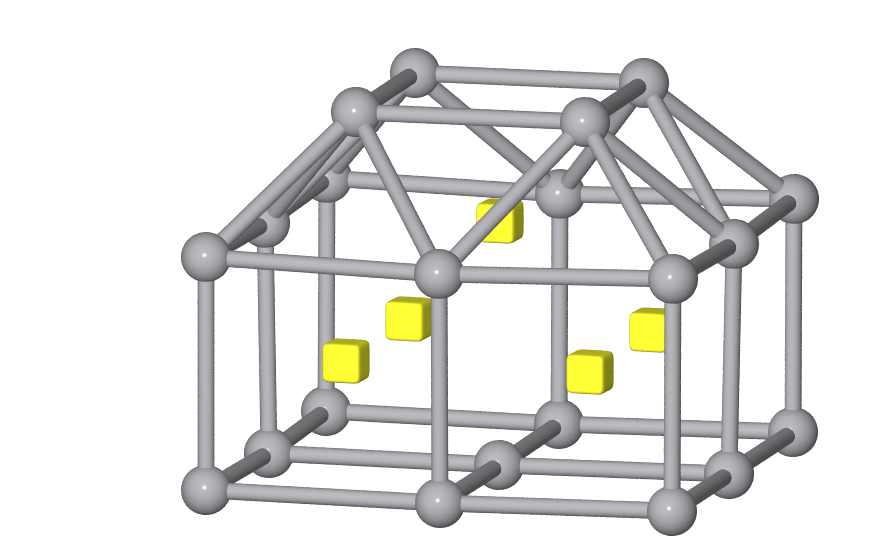
\includegraphics[scale=0.1]{figures/V/v5.png} \\
    (d) & (e) & (f) \\
 \end{tabular}
\caption{The configurations of vacancy clusters ($V_m$, $m=1, 2, 3, 4,5 $) with the lowest formation energy. 
For the case of di-vacancy we plot the first nearest neighbour ($V_2^{1nn}$) and the second nearest neighbour 
configuration $V_2^{2nn}$: (a) $V_1$, (b) $V_{2}^{1nn}$, (c) $V_{2}^{2nn}$, (d) $V_3$, (e) $V_4$, (f) $V_5$.
The vacancies are represented by cubes while the atoms of the bcc lattice are represented with spheres. \label{fig:vacancies}}
\end{center}
\end{figure}

The formation energy for mixed He-vacancy clusters, He$_nV_m$ (up to \textit{n}=26 for \textit{m}=4),  is defined as :
%
\begin{equation}
 E^f_{He_nV_m} = E_{He_nV_m} - \dfrac{(N-m)}{N} \times E_0 - n\times E_{He}
 \label{eq:form}
\end{equation}
%
where E$_{He_nV_m}$ is the DFT energy of the supercell containing the He$_n$V$_m$ cluster.
%construction of clusters 
The construction of clusters for a given number of $n$ He atoms and $m$ vacancies is not simple task. 
The number of possible choice grows as  exponential with the number of defects and He atoms, consequently, 
several choices should be made in order to choose the initial geometries of those configurations.  
He atoms have been chosen as strategy that for any given  He$_nV_m$ cluster the $n$ He atoms decorate the most $V_m$ stable 
clusters, deduced previously and presented in the Fig.~\ref{fig:vacancies}. 
The only exception was the di-vacancy for which the two configurations first and second nearest neighbours have been chosen.   
%number of choices ... 
Moreover for a given $n$ and $m$ we picked randomly tens of configurations, for which the He atoms were placed at first nearest neighbour 
$T$, $O$ or substitutional ($S$) sites to the vacancy.
Nevertheless, we should highlight that considering the restricted sample taken within the many possible isomers, 
there is no guarantee we selected the most stable clusters, in particular for the largest clusters. 
But, for the smallest clusters we can be reasonably confident in finding the lowest energy configurations.

For mixed configurations He$_1V_1$ in V, the  lowest energy configuration is given  by the He atom 
slightly off $O$ site, as it presented in Fig.~\ref{fig:henv1} with the formation energy of 4.47 eV. 
The $S$ configuration is higher in energy with 0.21 eV. 
In Ta, the $S$ site is the only found stable configuration. 
All calculations having as the initial position as $T$ and $O$ position of He are finally relaxed into 
the $S$ configuration.  


\begin{figure}
% \begin{adjustwidth}{-2cm}{}
% \resizebox{1\columnwidth}{!}{%
\begin{center}
 \begin{tabular}{ccccc}
    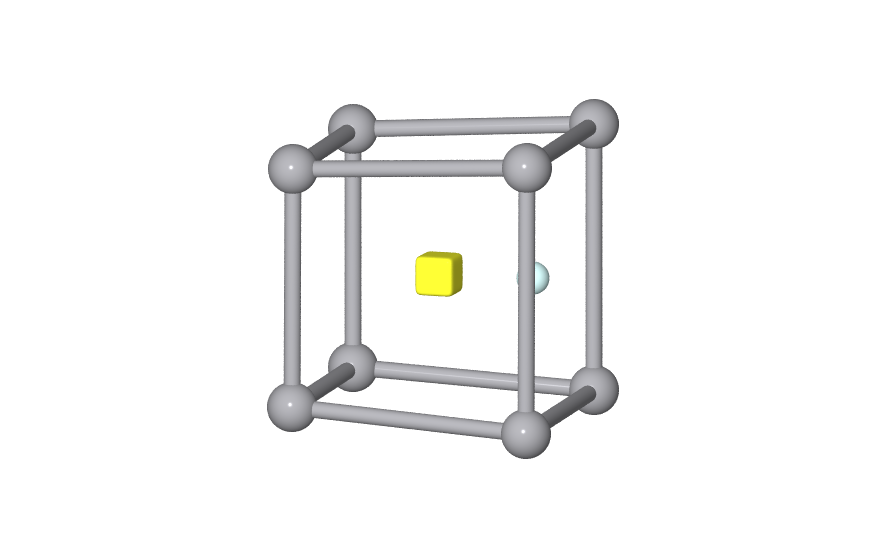
\includegraphics[scale=0.1]{figures/V/he1v1_octa.png} &
    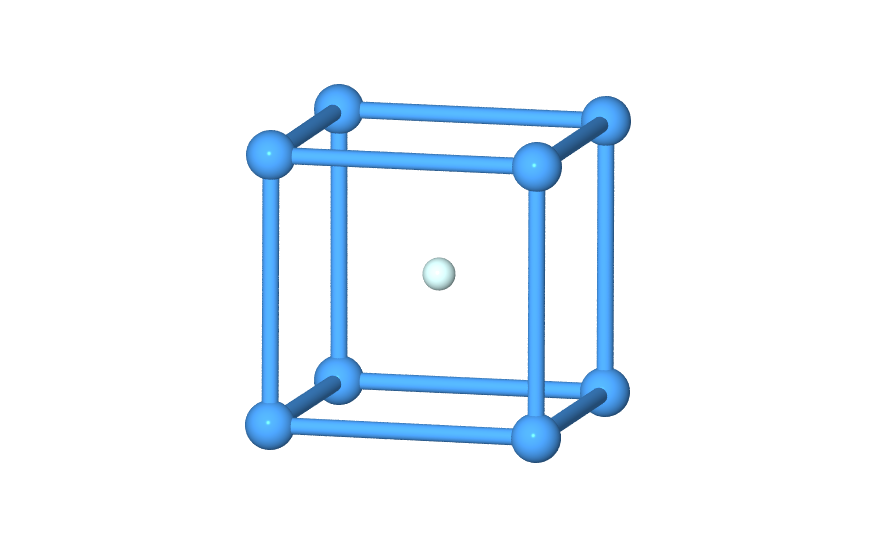
\includegraphics[scale=0.1]{figures/Ta/he1v1.png} &
    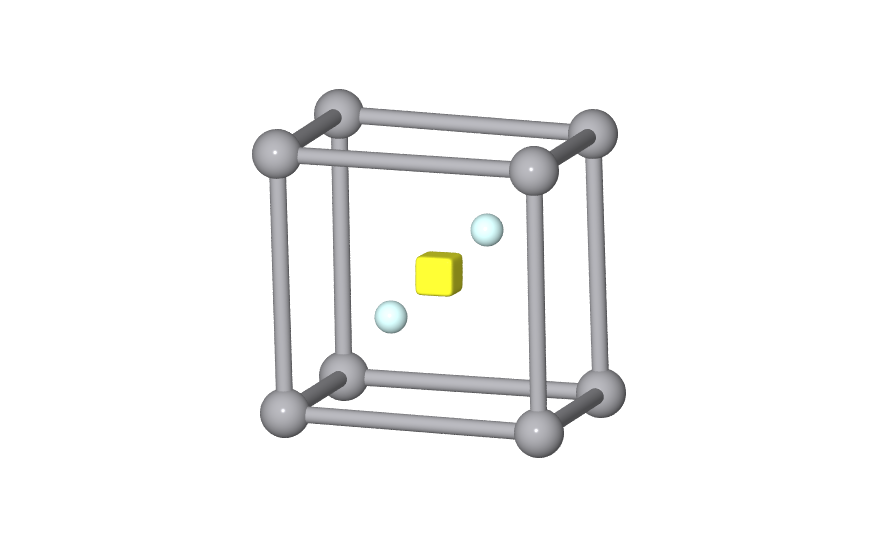
\includegraphics[scale=0.1]{figures/V/he2v1_111.png} &
    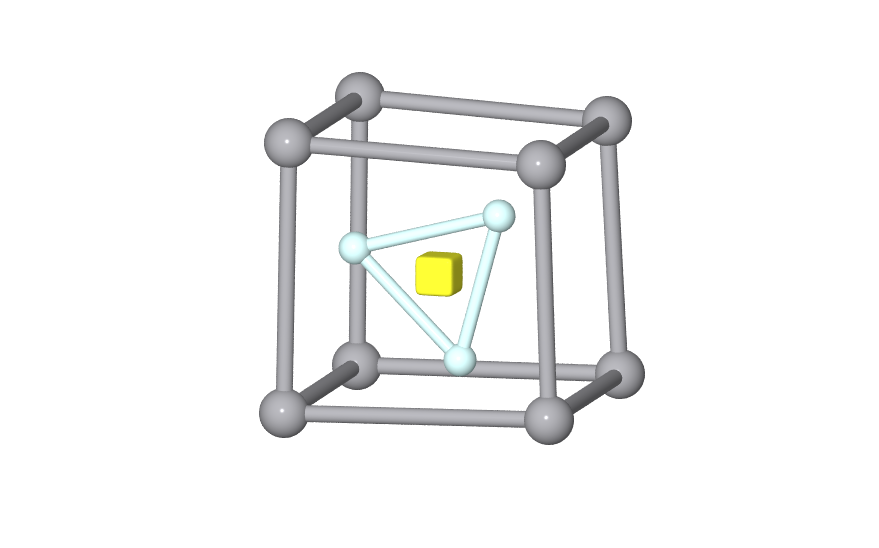
\includegraphics[scale=0.1]{figures/V/he3v1_oso.png} &
    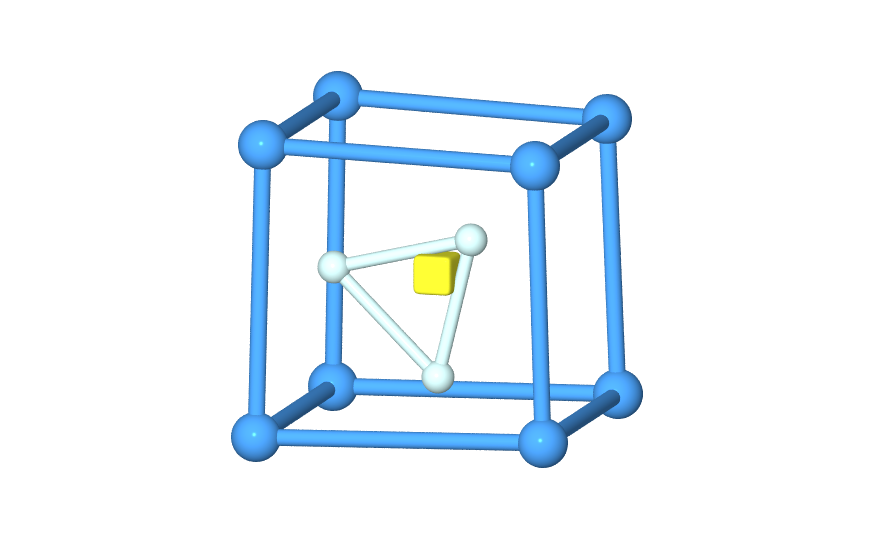
\includegraphics[scale=0.1]{figures/Ta/he3v1.png} \\
    \multicolumn{2}{c}{(a)} & (b) & \multicolumn{2}{c}{(c)} \\
    &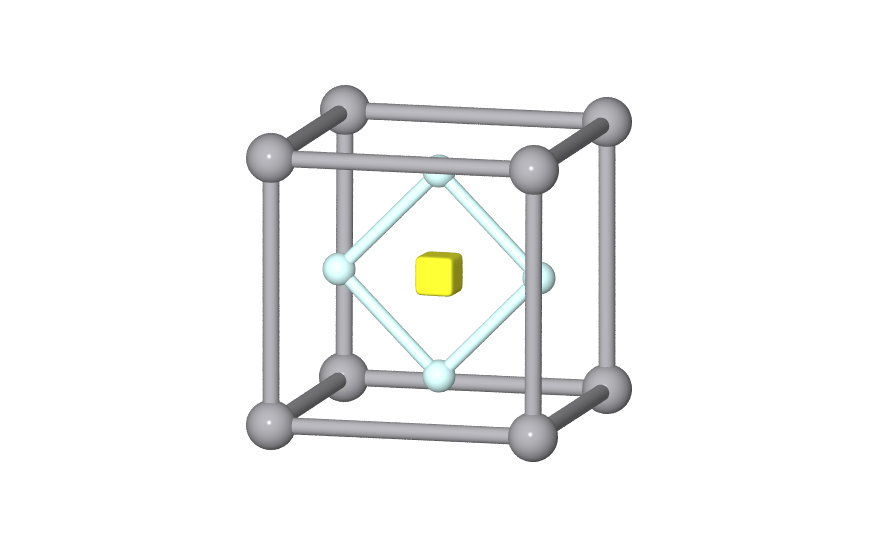
\includegraphics[scale=0.1]{figures/V/he4v1_4o.png} &
    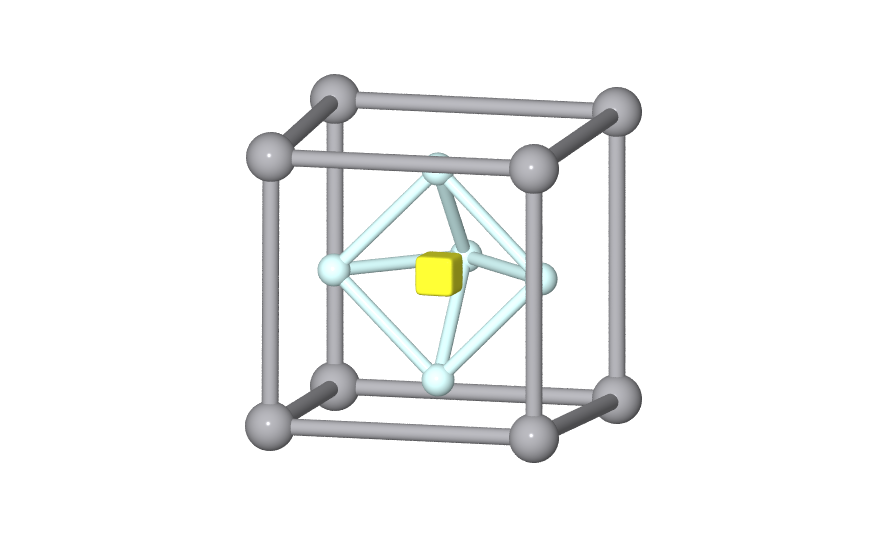
\includegraphics[scale=0.1]{figures/V/he5v1_5o.png} &
    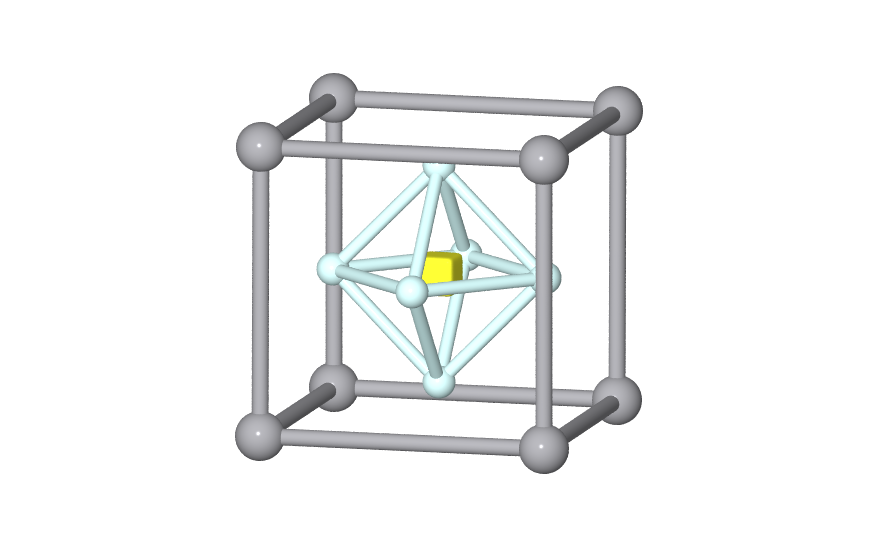
\includegraphics[scale=0.1]{figures/V/he6v1_6o.png} &\\
    & (d) & (e) & (f) & \\
 \end{tabular}
 \caption{Lowest formation energy He$_nV_1$ type clusters in V and Ta. 
 (a) He$_1V_1$, (b) He$_2V_1$, (c) He$_3V_1$, (d) He$_4V_1$, (e) He$_5V_1$, (f) He$_6V_1$. 
 Vacancy is represented with yellow cube, V with grey ball, Ta with dark blue ball and 
 helium with light blue ball. Configurations for Ta are shown only when different to V ones.\label{fig:henv1}}
%  \end{adjustwidth}
\end{center}
\end{figure}


For clusters with 2 He atoms, He$_2V_1$, the impurities and the vacancy cluster are aligned along 
the $\langle 111 \rangle$ direction for both V and Ta.
One can notice in case of He$_3V_1$ cluster, He atoms form an equilateral triangle centered on the vacancy in V, 
while in Ta, a He atom is shifted toward the vacancy and the 2 others occupy positions closed to $O$ sites 
(Fig.~\ref{fig:henv1} c).
%
The geometry of clusters with the lowest formation energy  from \textit{n}=4 to \textit{n}=6 have all 
He atoms close to $O$ sites in both V and Ta case.
In V, for di-vacancy clusters, He$_1V_2$,  the $1nn$ configuration is still higher in energy 
than in the $2nn$ configuration (Fig.\ref{fig:henv2}). 
However, the difference is reduced to 0.09 eV compared to 0.19 eV in the pure vacancy, $V_2$, cluster (Tab.\ref{tab:efv}). 
%
\begin{figure}
 \begin{tabular}{cccc}
    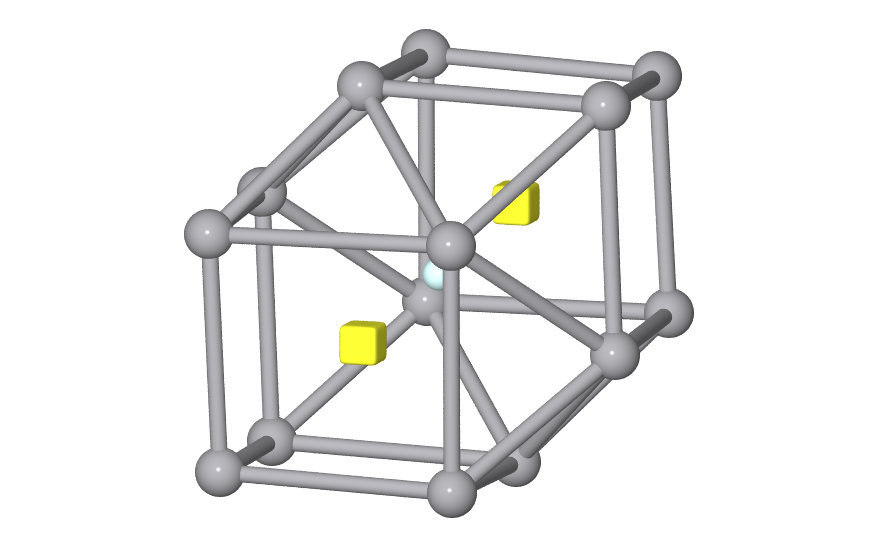
\includegraphics[scale=0.1]{figures/V/he1v2a_111.png} &
    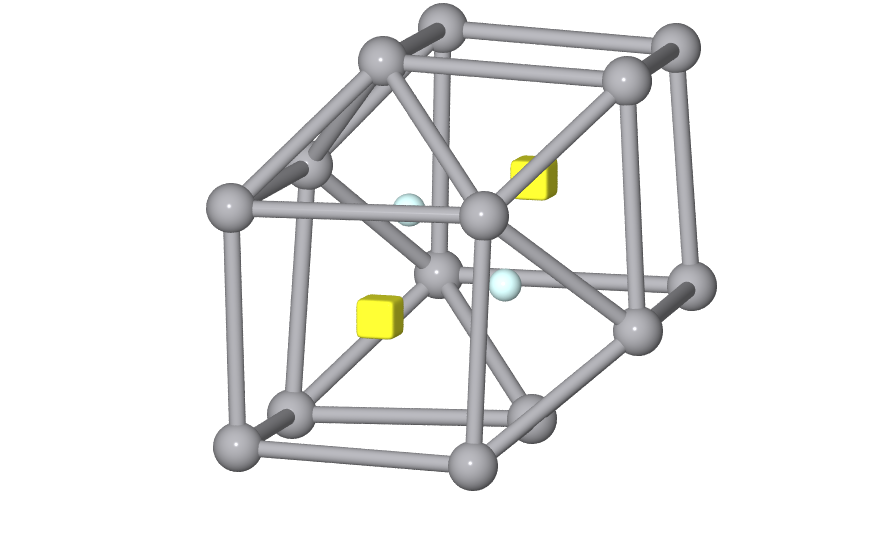
\includegraphics[scale=0.1]{figures/V/he2v2a_2o.png} &
    
\includegraphics[scale=0.1]{figures/V/he3v2a.png} &
    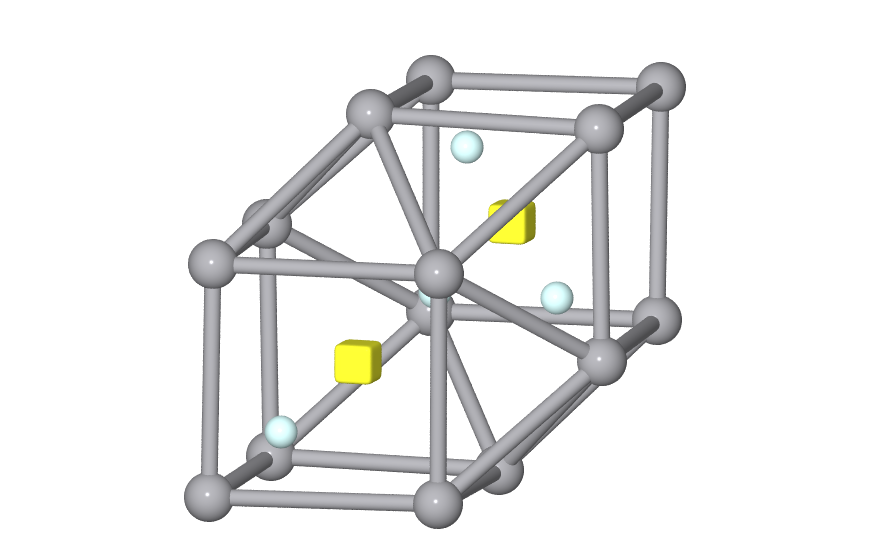
\includegraphics[scale=0.1]{figures/V/he4v2a_111.png} \\
    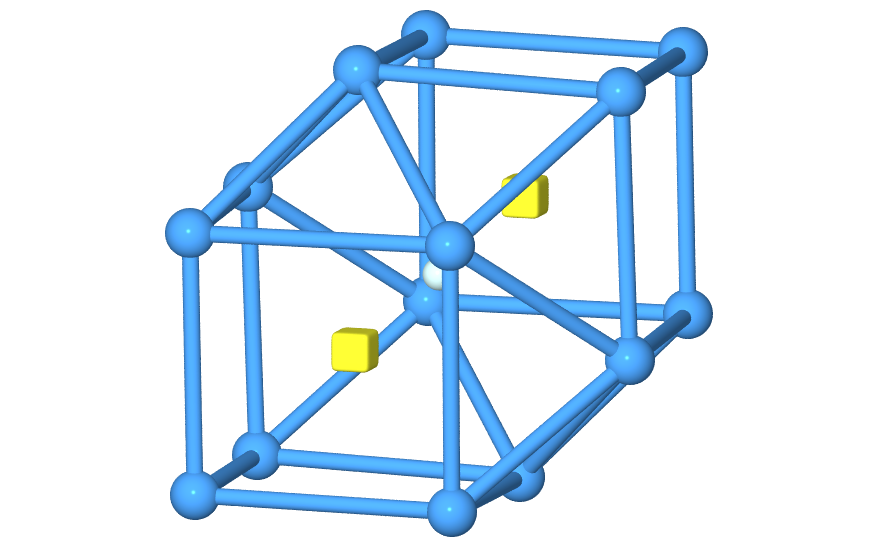
\includegraphics[scale=0.1]{figures/Ta/he1v2a.png} &
    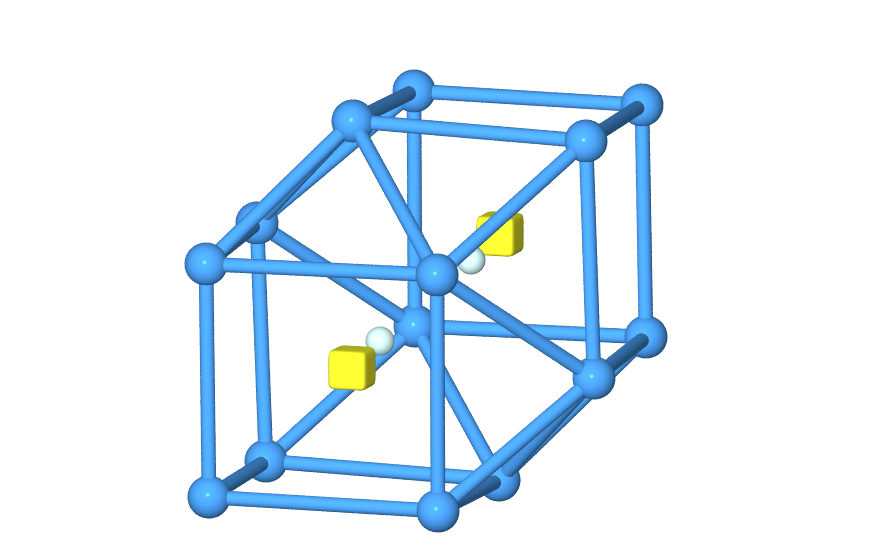
\includegraphics[scale=0.1]{figures/Ta/he2v2a.png} &
    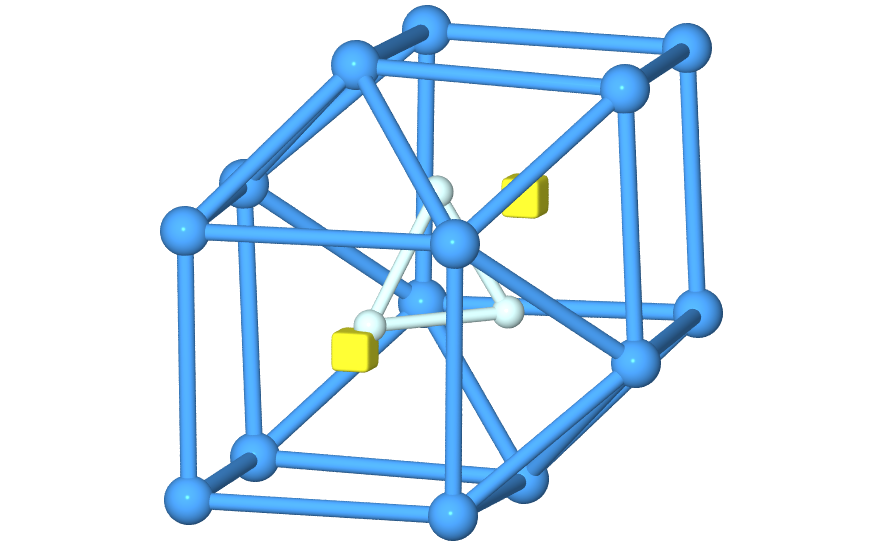
\includegraphics[scale=0.1]{figures/Ta/he3v2a.png} &
    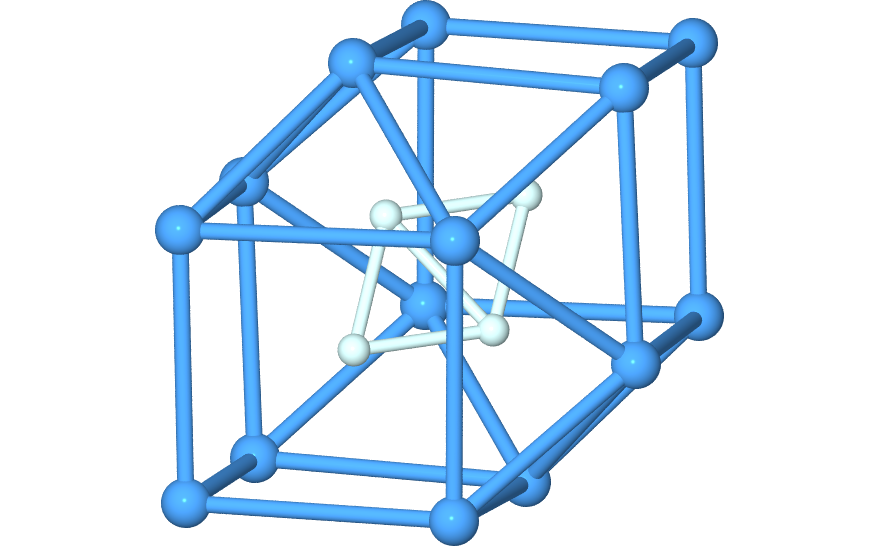
\includegraphics[scale=0.1]{figures/Ta/he4v2a.png} \\
    (a) & (b) & (c) & (d) \\
    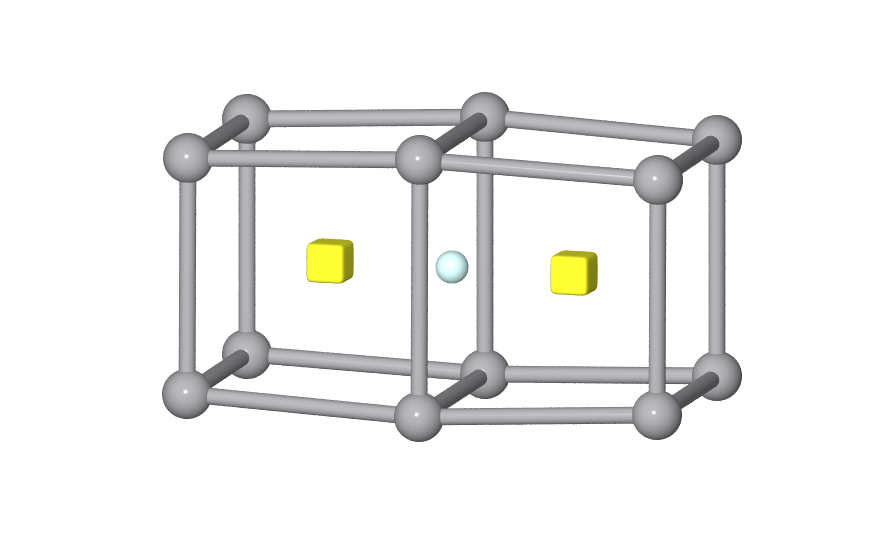
\includegraphics[scale=0.1]{figures/V/he1v2b_octa.png} &
    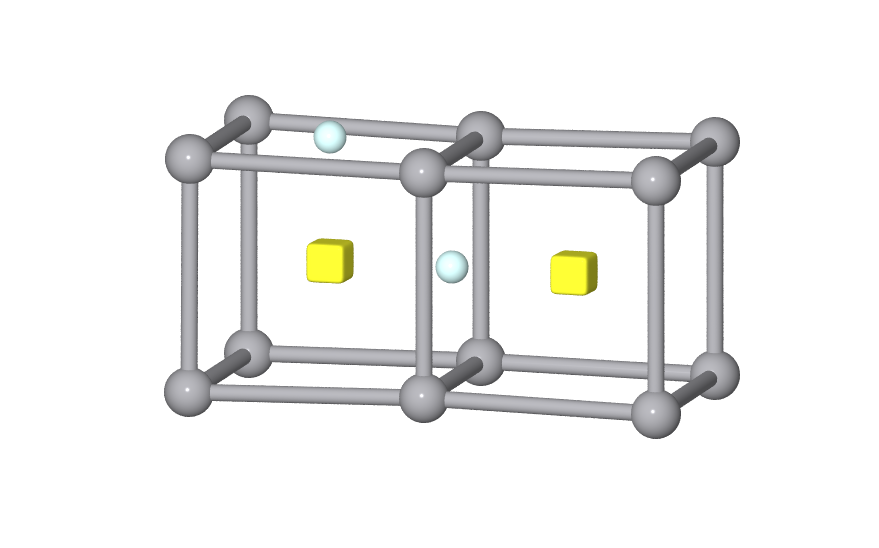
\includegraphics[scale=0.1]{figures/V/he2v2b_2o.png} &
    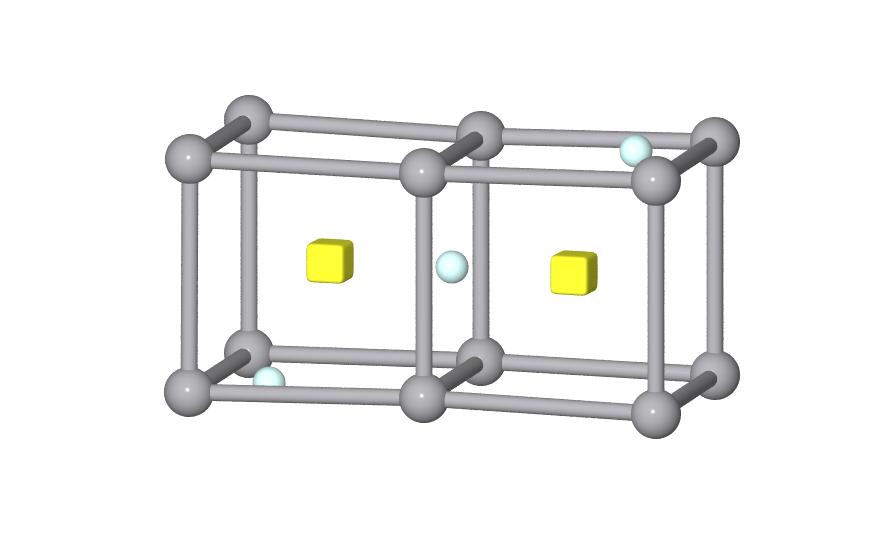
\includegraphics[scale=0.1]{figures/V/he3v2b_o2t.png} &
    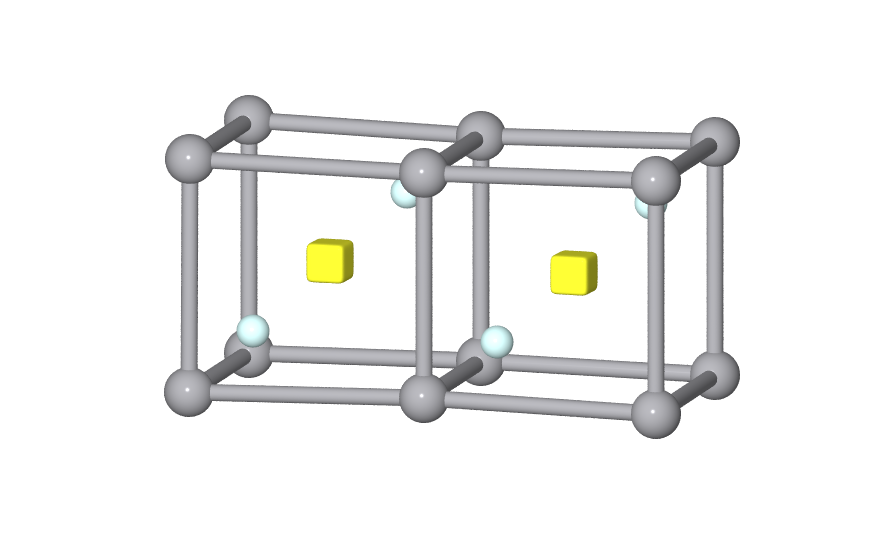
\includegraphics[scale=0.1]{figures/V/he4v2b_111.png} \\
    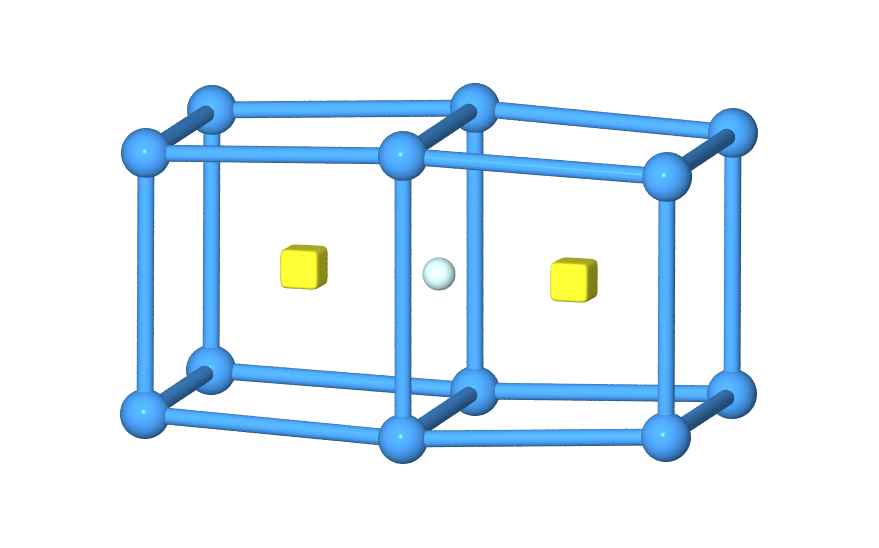
\includegraphics[scale=0.1]{figures/Ta/he1v2b.png} &
    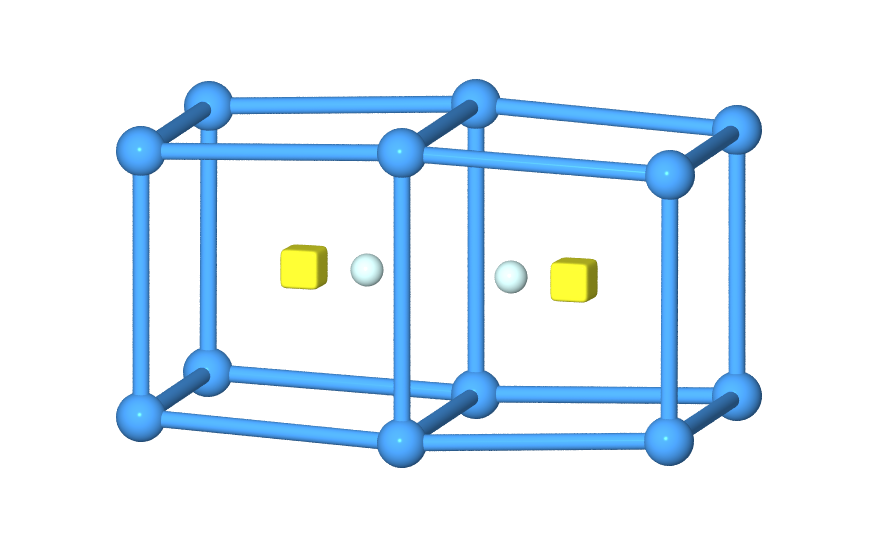
\includegraphics[scale=0.1]{figures/Ta/he2v2b.png} &
    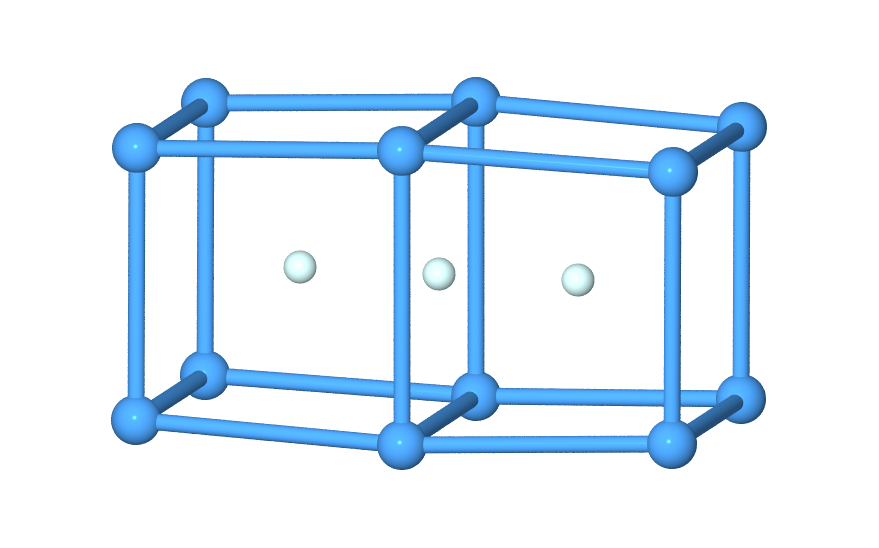
\includegraphics[scale=0.1]{figures/Ta/he3v2b.png} &
    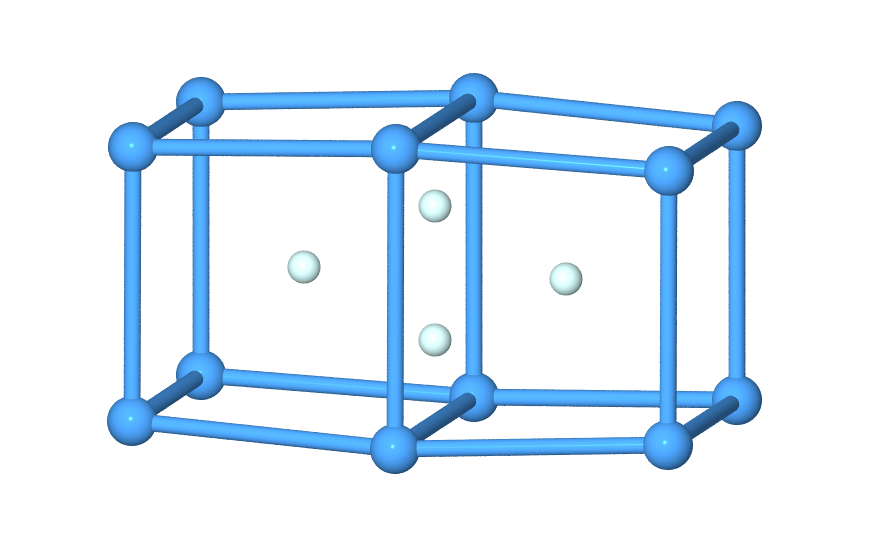
\includegraphics[scale=0.1]{figures/Ta/he4v2b.png} \\
    (e) & (f) & (g) & (h) \\
 \end{tabular}
 \caption{The geometries of the lowest formation energy clusters of the type He$_nV_2$  in V (grey bcc lattice) and Ta (blue bcc lattice). The geometry of the di-vacancy clusters are taken in first nearest neighbour (1nn) and the second nearest neighbour configuration.
 (a) He$_1V_{2}^{1nn}$, (b) He$_2V_{2}^{1nn}$, (c) He$_3V_{2}^{1nn}$, (d) He$_4V_{2}^{1nn}$, (e) He$_1V_{2}^{2nn}$, 
 (f) He$_6V_{2}^{2nn}$, (g) He$_3V_{2}^{2nn}$, (h) He$_4V_{2}^{2nn}$.
Vacancy and the He impurities are represented with yellow cube
and light blue spheres, respectively. 
When the He atom is placed in the $S$ site the corresponding vacancy cube is not plotted. \label{fig:henv2}}
\end{figure}
%


Adding more He diminishes the formation energy difference between 1nn and 2nn configuration up to $n$=1. 
For $n \ge 2$ the formation of the 1nn configuration requires less energy than the 2nn one.

In Ta, except for the case of di-vacancy without He, the formation energy of 1nn configuration is 
systematically less than for the 2nn case. Futhermore, the energy difference between these two configurations is larger 
when adding more He atoms.

Comparing the energy landscape of He in the neighborhood of the vacancy in V and Ta, it can be notted that 
the $S$ site is attractive in Ta while it is repulsive in V (Fig.\ref{fig:henv1}--\ref{fig:henv2}). 
Similar result has been found \cite{seletskaia2008} which explain this tendency by a larger charge density at vacancy 
in V than in Ta. The energy of electronic charge in the vacancy is close to the Fermi level. 
In addition, He \textit{s}-state at vacancy have a larger density of state at Fermi level in V than in Ta, so He will have 
a stronger repulsive interaction at $S$ site in V, 
increasing the formation energy enough to make this configuration unstable. 
As a result in the most stable configuration, He is shifted toward $O$ site.

 \begin{table}
 \centering
 \begin{tabular}{c|cccccc|cccccc}
 
  & \multicolumn{6}{c|}{V} & \multicolumn{6}{c}{Ta} \\
 \hline \hline
 \diag{.1em}{.5cm}{n}{m} & 0 & 1 & 2 (1nn) & 2 (2nn) & 3 & 4 & 0 & 1 & 2 (1nn) & 2 (2nn) & 3 & 4\\
\hline \hline
 0 & & 2.47 & 4.69 & 4.50 & 6.46 & 8.07 & & 2.88 & 5.66 & 5.42 & 7.97 & 9.96\\ 
   & & (2.1\textpm 0.2)$^a$ & & & & & & (2.8\textpm0.6)$^a$ & & & \\
   & & (2.2\textpm 0.4)$^b$ & & & & & & (3.1)$^c$ & & & & \\
   & & & & & & & & (2.9\textpm0.4)$^d$ & & & & \\
 1 & 3.12 & 4.47 & 6.15 &  6.06 & 7.58 & 8.88 & 3.47 & 4.66 & 6.89 & 6.92 & 8.77 & 10.44\\
 2 & 6.16 & 6.26 & 7.54 & 7.94 & 8.90 &  9.81 & 6.84 & 6.49 & 8.22 & 8.40 & 9.97 & 11.31\\
 3 & 9.15 & 8.15 & 9.18 &  9.74 & 10.09 & 10.84 & 10.00 & 8.63 & 9.69 & 10.07 & 11.09 & 12.28\\
 4 & 12.03 & 10.01 & 10.92 & 11.48 & 11.74 & 11.92 & 13.26 & 10.79 & 11.22 & 11.80 & 12.29 & 13.31\\
 5 & & 11.91 & 12.47 & 13.45 & 12.99 & 13.20 &  & & 12.84 & 14.19 & 13.81 & 14.46\\
 6 & & 13.73 & 14.44 &  15.07 & 14.62 & 14.76 & & 14.87 & 14.80 & 15.69 & 15.39 & 15.62\\
  \hline \hline
 \end{tabular} 
 \caption{\label{tab:efv}
 The lower limit of formation energy (in eV) of He$_nV_m$ clusters, 
 extracted from the present calculations, using Eq.~\ref{eq:form},  
 for small values of $n$ and $m$.\\
 $^a$ Experimental data from Ref \cite{maier1979}\\ $^b$ Experimental data from Ref \cite{janot1982}\\
 $^c$ Experimental data from Ref \cite{schultz1982}\\ $^d$ Experimental data from Ref \cite{Schaefer1987}
 }
  \end{table}
  
  
For all types of cluster He$_nV_m$, the cost in energy to form He$_{n+1}V_m$ increases linearly with \textit{n} 
but the slope decreases with \textit{m} (see Fig.\ref{fig:formation_slope}). 
\wes{This linear behaviour of formation energy with $n$ can be explained by the fact that the He is weakly bound to He$_n$ clusters 
whereas He-vacancy binding energy is 1-2 order of magnitude larger (Tab.\ref{tab:ebhe}). Hence, adding a He atom result in adding one more 
He-vacancy interaction, until the vacancy is filled with He.
Also the slope decreases with \textit{m} since He atoms have more space to maximize He-He distance.
According to Ref.\cite{Zhang2015}, for group $VB$ metals such as V and Ta, He-He interaction is weaker and He-He distance is larger 
than for group $VIB$ transition metal (W, Mo). 
As a consequence, one can expect an inflection in the linear law for these group $VIB$ metals for smaller clusters than for 
group $VB$.}
\MCM{We should explain why. He-He bound compared to the vacancy-He? Is someho expected bu we should provide more details} 

\begin{figure}
 \centering
  \begin{tabular}{cc}
 
\includegraphics[scale=0.35]{figures/V/E_f.png}&
 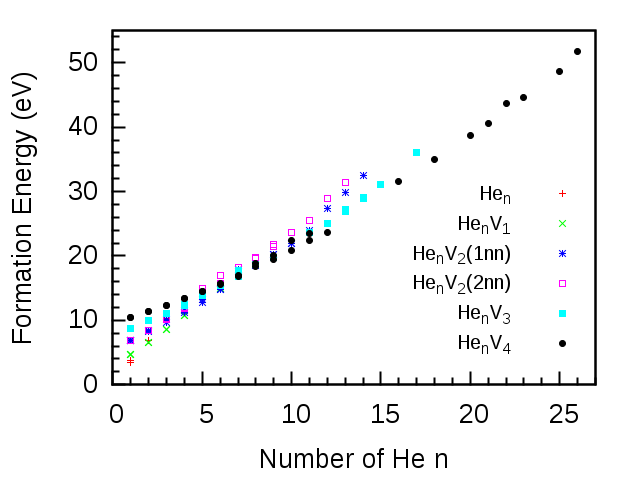
\includegraphics[scale=0.35]{figures/Ta/E_f.png}\\
 \multicolumn{2}{c}{
%  \resizebox{0.6\columnwidth}{!}{%
  \begin{tabular}{c|c|cccccc}
  \hline
     & m & 0 & 1 & 2 (1nn) & 2 (2nn) & 3 & 4\\ \hline
   V & $\Delta$E$^f_{n \rightarrow n+1}$ (eV) & 2.97 & 1.86-2.05 & 1.76-1.82 & 1.81-1.88 & 1.63 & 1.51-1.66\\ \hline 
   Ta & $\Delta$E$^f_{n \rightarrow n+1}$ (eV) & 3.26 & 2.06 & 1.73-2.19 & 1.87-2.10 & 1.41-1.90 & 1.07-1.35 \\ \hline 
 \end{tabular}}\\
 \end{tabular}
 \caption{\label{fig:formation_slope}
 In the upper graph we present the formation energy (in eV) of clusters He$_nV_m$ as a function of \textit{n}, number of He atoms, in V (left panel) and Ta (right panel). For di-vacancy clusters the labels $1nn$ and $2nn$ stand for di-vacancy configurations in first nearest neighbour and second nearest neighbour, respectively.
The lower table gives the slope for each type of cluster, at fixed $m$. In the case when two values are presented, we give the upper and lower limit of possibles choices of slope.}
 \end{figure}



\subsection{Stability of He--vacancy clusters}\label{binding}
We investigated the stability of pure He and vacancy clusters and He--vacancy complexes 
looking at their binding energy to helium atom and mono-vacancy given respectively by :
%
\begin{equation}
E^b_{He-He_nV_m} = E_{He_I} + E_{He_{n-1}V_m} - E_{He_nV_m} - E_0 
\label{eq:bind:he}
\end{equation}
%
and
%
\begin{equation}
  E^b_{V-He_nV_m} = E_V + E_{He_nV_{m-1}} - E_{He_nV_m} - E_0
\label{eq:bind:v}
\end{equation}
%
where  $E_{He_I}$ is the total energy of the bcc supercell in which is inserted an interstitial He at $T$ or $S$ site for V and Ta, respectively.
% 
$E_V$ is the total energy of the bcc supercell with one mono-vacancy.

Following Eqs.~\ref{eq:bind:he} and~\ref{eq:bind:v}, positive binding energy corresponds to an attractive interaction for He and vacancy, respectively.  
Therefore the clusters with the highest binding energy are more stable.
%
The Fig.\ref{fig:eb_he} emphasizes a general overview of the binding energy of one He atoms in the clusters He$_nV_m$ for V and Ta. 
Firstly, it should be noted the broad distribution in He binding energy for the same type of cluster i.e. fixed number of $n$ and $m$.  
The sparse values of the binding energy indicate a strong dependence on the cluster morphology. 
For each pair of $n$ and $m$ there are wide variety of clusters in which He is strongly or weakly bound. 
For practical use, e.g. in cluster dynamics simulations,  in first order approximation are important only 
the upper value of those binding energies. The values are extracted in Tab.~\ref{tab:ebhe}.  
The thermal equilibrium conditions  will select only the most stable, the excited configurations having a influence only as second order e.g. through the configurational entropy.     
%
In V, the binding energy of He in pure He$_n$ clusters range from -0.38 eV to 0.24 eV, slowly increasing with the amount of He 
at least up to \textit{n}=4, similar to Ta case. 
%
We note that in V and Ta the binding energy of He in He$_4$ clusters is almost 4 times lower than for the similar clusters in Fe ($\sim$1 eV)\cite{Fu2005}
%
Adding more He in interstitial clusters He$_n$ at least up to $n$=4, amplifies lattice distorsion so that 
the increasing pressure may lead to the creation of 
Frenkel pair as predicted in Fe \cite{FU2008335,Morishita2003,wilson1981} and observed in Ni \cite{thomas1979} 
and Au \cite{thomas1981}. This idea is supported by the lower formation energy for He$_{n}V_1$ clusters
than for He$_{n}$ interstitial clusters for $n\ge3$ in V and $n\ge2$ in Ta (Tab.\ref{tab:efv}).
%

The upper limit of the He binding energy in He$_nV_m$ at given \textit{n}, 
increases with the number of vacancies. This tendency can be remarked from the Tab.~\ref{tab:ebhe}.
% 
A second trend which can be identified at first glance is that a given \textit{m}, 
the He binding energy seems to decrease with \textit{n}, especially for V$_3$ (Fig.\ref{fig:eb_he})
With the same increasing $n$ we expect an increase in the  internal pressure of the cavity created by vacancies.  
Therefore, spontaneous emission of He or self-interstitial, V or Ta atoms, may occurs for large \textit{n/m} ratio \cite{SUBRAHMANYAM1996,SUBRAHMANYAM1995}
This behaviour has been observed at low temperature by Fedorov~\cite{Fedorov1996} in V and V alloys, 
and also theoretically predicted in Fe by Morishita~\cite{Morishita2003}.
 
But a closer look reveals for \textit{m}=1, in V, 
the binding energy seems to saturate (up to \textit{n}=6) indicating that more He atoms can be added 
before internal pressure reach a threshold such that significant drop in the binding energy occurs. 
Indeed, previous calculations showed mono-vacancy clusters with tens of He atoms still have attractive interaction 
with He \cite{Li2013}.
This apparently drop in the binding energy with $n$, may reflect the fact we missed more stable clusters in our sampling.
In the di-vacancy case, we see again that He make the He$_nV_2^{1nn}$ clusters more stable than the 
He$_nV_{2}^{2nn}$ ones when we have the opposite situation without He.
%
In both V and Ta, He$_8V_{2}^{1nn}$ seem particularly stable compared to He$_7V_{2}^{1nn}$ and He$_9V_{2}^{1nn}$. 
In the He$_8V_{2}^{1nn}$ clusters He atoms occupy high symmetry interstitial sites $O$ and $T$ 
while the position of He is more shifted from $O$ and $T$ sites in He$_7V_{2}^{1nn}$ and He$_9V_{2}^{1nn}$.
Corrolary, in V, H$_{20}V_4$ clusters which are clearly unstable with negative binding energy, 
contrary to  He$_{19}V_4$ and  He$_{21}V_4$ clusters for which more high symmetry sites are occupied by He atoms.

\begin{table}
 \centering
 \begin{tabular}{c|cccccc|cccccc}
 
  & \multicolumn{6}{c}{V} & \multicolumn{6}{c}{Ta} \\
 \hline \hline
 \diag{.1em}{.5cm}{n}{m}  & 0 &  1 & 2 (1nn) & 2 (2nn) & 3 & 4 & 0 & 1 & 2 (1nn) & 2 (2nn) & 3 & 4\\
 \hline \hline
 1 & 0.01 & 1.12 & 1.64 & 1.50 & 2.01 & 2.32 & 0.01 & 1.75 & 2.22 & 1.95 & 2.66 & 2.97\\
 2 & 0.09 & 1.34 & 1.73 & 1.24 & 1.81 & 2.21 & 0.06 & 1.62 & 2.00 & 1.98 & 2.25 & 2.58\\
 3 & 0.14 & 1.24 & 1.49 & 1.33 & 1.94 & 2.10 & 0.30 & 1.32 & 2.11 & 1.77 & 2.33 & 2.49\\
 4 & 0.24 & 1.26 & 1.39 & 1.38 & 1.48 & 2.04 & 0.20 & 1.29 & 1.92 & 1.72 & 2.25 & 2.42\\
 5 & & 1.23 & 1.58 & 1.16 & 1.87 & 1.85 & &  & 1.84 & 1.07 & 1.93 & 2.31\\
 6 & & 1.30 & 1.16 & 1.51 & 1.50 & 1.57 & &  & 1.49 & 1.95 & 1.87 & 2.29\\
  \hline \hline
 \end{tabular} 
 \caption{\label{tab:ebhe}
 The upper limit of binding energy (in eV) of He to He$_nV_m$ clusters, 
 extracted from the present calculations, using Eq.~\ref{eq:bind:he},  
 small values of $n$ and $m$.}
\end{table}


\begin{figure}
\centering
\begin{tabular}{cc}
 
\includegraphics[scale=0.35]{figures/V/E_b_He-He_nV_m.png} &
%  \caption{Binding energy of He to He$_n$V$_m$ clusters as a function of \textit{n} in V\label{fig:V_eb_he}}
% \end{figure}

% \begin{figure}
% \centering
 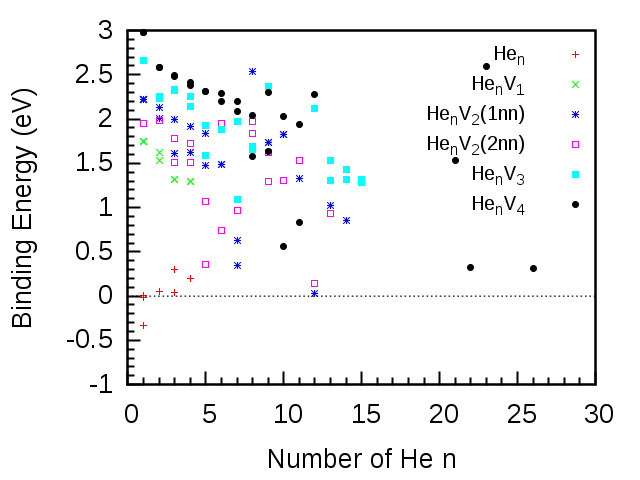
\includegraphics[scale=0.35]{figures/Ta/E_b_He-He_nV_m.png}\\
%  \caption{Binding energy of He to He$_n$V$_m$ clusters as a function of \textit{n} in Ta\label{fig:Ta_eb_he}}
 \end{tabular} 
 \caption{Binding energy of He to He$_nV_m$ clusters as a function of \textit{n} in  V (left panel) 
 and Ta (right panel)\label{fig:eb_he}}
\end{figure}

 \begin{table}
 \centering
 \begin{tabular}{c|ccccc|ccccc}
 
  & \multicolumn{5}{c}{V} & \multicolumn{5}{c}{Ta} \\
 \hline \hline
 \diag{.1em}{.5cm}{n}{m}  & 1 & 2 (1nn) & 2 (2nn) & 3 & 4 & 1 & 2 (1nn) & 2 (2nn) & 3 & 4\\
 \hline \hline
 0 & 0.00 & 0.27 & 0.51 & 0.43 & 0.87 & 0.00 & 0.26 & 0.50 & 0.40 & 0.97\\
 1 & 1.11 & 0.79 & 0.89 & 0.94 & 1.17 & 1.74 & 0.73 & 0.70 & 1.11 & 1.28\\
 2 & 2.37 & 1.19 & 0.79 & 1.50 & 1.57 & 3.31 & 1.11 & 1.06 & 1.39 & 1.61\\
 3 & 3.47 & 1.43 & 0.88 & 2.12 & 1.72 & 4.33 & 1.90 & 1.51 & 1.94 & 1.77\\
 4 & 4.49 & 1.56 & 1.00 & 2.22 & 2.28 & 5.43 & 2.52 & 1.94 & 2.47 & 1.93\\
 5 &  & 1.91 & 0.92 & 2.93 & 2.25 &  &  &  & 3.33 & 2.32\\
 6 &  & 1.76 & 1.13 & 2.92 & 2.32 & & 3.02 & 2.14 & 3.26 & 2.73\\
  \hline \hline
 \end{tabular} 
 \caption{The upper limit of binding energy (in eV) of vacancy to He$_nV_m$ clusters, 
 extracted from the present calculations, using Eq.~\ref{eq:bind:v},  
 small values of $n$ and $m$.\label{tab:ebv}}
\end{table}

 
The binding energy of vacancy in pure vacancy clusters $V_m$ increases with the number of vacancy 
from 0.27 eV to 0.88 eV in V (Fig.\ref{fig:eb_v}). 
It seems to reach a plateau at \textit{m}=4 around 0.87 eV. 
Similar behaviour has been reported in Fe, using molecular dynamics simulation for which 
the binding energy saturates slightly above 1 eV for \textit{m} $\gtrsim$ 20 \cite{Morishita2003}.
But for Ta, the binding energy of vacancy is likely to be linear at least up to $m$=4 with corresponding energy 0.97 eV.


From the values presented in the Tab.~\ref{tab:ebv}, the presence of He atoms in vacancy clusters enhances 
the binding energy to mono-vacancy, reflecting the fact that He stabilizes vacancy type clusters. 
We find again He$_nV_{2}^{1nn}$ are more stable than He$_nV_{2}^{2nn}$ for n $\ge$ 2 and  n $\ge$ 1 in V and in Ta, respectively.

\begin{figure}
\centering
\begin{tabular}{cc}
 
\includegraphics[scale=0.35]{figures/V/E_b_V-He_nV_m.png}&
%  \caption{Binding energy of mono-vacancy to He$_n$V$_m$ clusters as a function of \textit{m} in V\label{fig:V_eb_v}}
% \end{figure}

% \begin{figure}
% \centering
 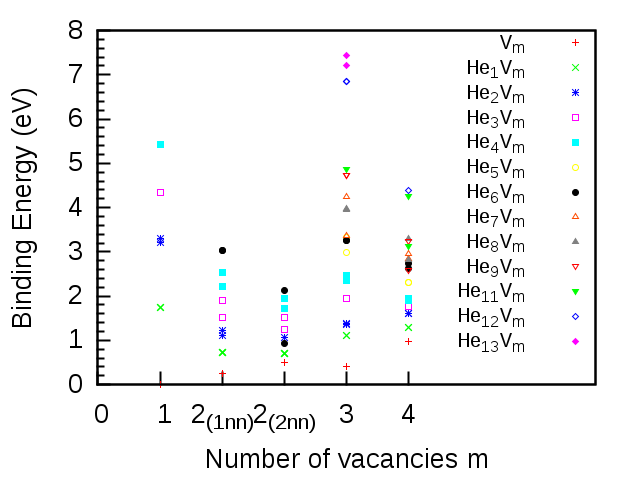
\includegraphics[scale=0.35]{figures/Ta/E_b_V-He_nV_m.png}\\
 \end{tabular}
 \caption{Binding energy of mono-vacancy to He$_nV_m$ clusters as a function of \textit{m} in V (left panel) 
 and Ta (right panel)
 \label{fig:eb_v}}
\end{figure}


\subsection{Migration energy barriers}\label{migration}

It is necessary to capture the diffusion processes of interstitial He and vacancy in order to 
understand how clusters grow at the primary stages. 
\wes{In the following, we restrict the scope of migration of vacancies toward their 1st nearest neighbour, 
i.e. in $\langle$111$\rangle$ direction.}


\subsubsection*{Vanadium}

We computed 2 paths for interstitial diffusion barrier that connect the lowest energy configurations : 
$T$ site to $T$ site, and $T$ site to $O$ site.
%
$T$ $\rightarrow$ $T$ path shows a barrier of 0.12 eV (Tab.\ref{tab:em}) in good agreement with TDS experiment 
in vanadium which gives the value of  0.13 eV~\cite{Fedorov1996}.
The barrier of this migration mechanism is twice than the similar migration barrier of He in Fe~\cite{Fu2005}.
%
The barrier of the migration path of He,  $T$ $\rightarrow$ $O$,  had the value 0.26 eV. 
Consequently, the interstitial He prefers to diffuse via through to first neighbour $T$ sites.



The DFT migration barrier of the mono-vacancy has the value of 0.48 eV and  agrees well with TDS experiments of Fedorov \cite{Fedorov1996}, 0.5 eV,  and van Veen,  0.47 eV, \cite{vanveen1994}.
\MCM{There is particular temperature for these experiments?}. 
The di-vacancy migration barrier from the $V_2^{1nn}$ configuration (Fig.\ref{fig:vacancies} b) 
to $V_2^{2nn}$ configuration (Fig.\ref{fig:vacancies} c) is 0.34 eV. 
The reverse way is less favored since the energy barrier is 0.58 eV.
Another path passing from a $V_2^{2nn}$ configuration to another $V_2^{2nn}$ configuration shows a barrier of 0.37 eV. 
This migration takes place within a 2 steps dissociation-recombination of vacancies process. 
One of the vacancy dissociates from the $V_2^{2nn}$ cluster to reach its 1st nearest neighbour position 
along the $\langle$111$\rangle$ direction. At this point the 2 vacancies are in a 4th nearest neighbour configuration 
(Fig.\ref{fig:mig:v2} b).
It is followed by the second vacancy that moves along a parallel $\langle$111$\rangle$ direction and 
recombines with the first vacancy to form again the $V_2^{2nn}$ cluster (Fig.\ref{fig:mig:v2} c).
\begin{figure}
 \begin{tabular}{ccc}
    
\includegraphics[scale=0.15]{figures/V/v2_btob/frame00.png} &
    
\includegraphics[scale=0.15]{figures/V/v2_btob/frame03.png} &
    
\includegraphics[scale=0.15]{figures/V/v2_btob/frame06.png} \\
    (a) & (b) & (c) \\
 \end{tabular}
 \caption{Di-vacancy migration along $V_{2}^{2nn}$ $\rightarrow$ $V_{2}^{2nn}$ path in V.
Vacancies are represented with yellow cube and V atom with grey ball.
When the metal atom is placed in the vacancy site the corresponding vacancy cube is not plotted\label{fig:mig:v2}}
\end{figure}

We turn on the influence of He on vacancy diffusion. 
%
\begin{figure}
 \begin{tabular}{ccccc}
    
\includegraphics[scale=0.1]{figures/V/v1he_seq/frame00.png} &
    
\includegraphics[scale=0.1]{figures/V/v1he_seq/frame03.png} &
    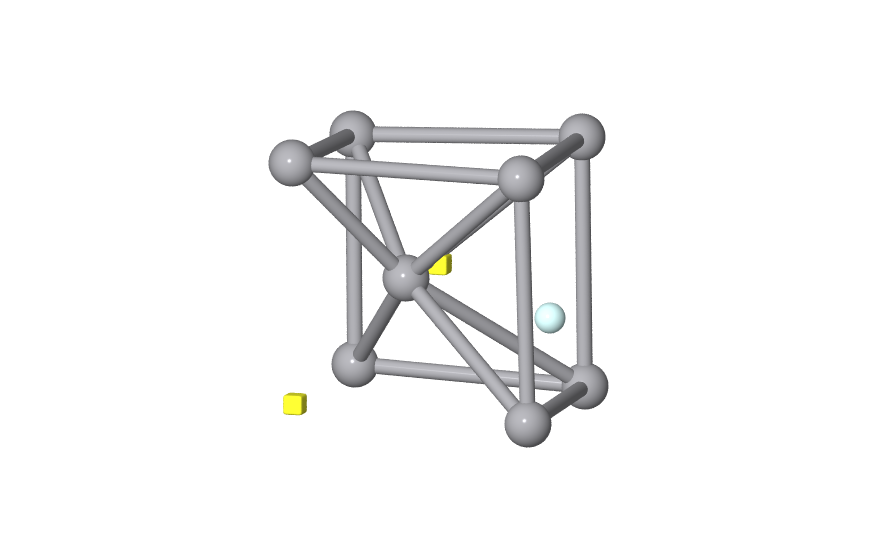
\includegraphics[scale=0.1]{figures/V/v1he_seq/frame09.png} &
    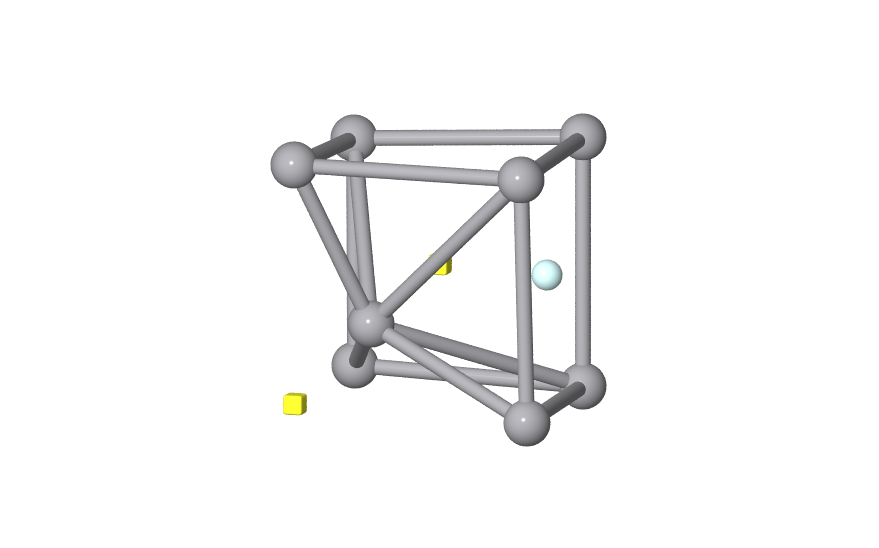
\includegraphics[scale=0.1]{figures/V/v1he_seq/frame11.png} &
    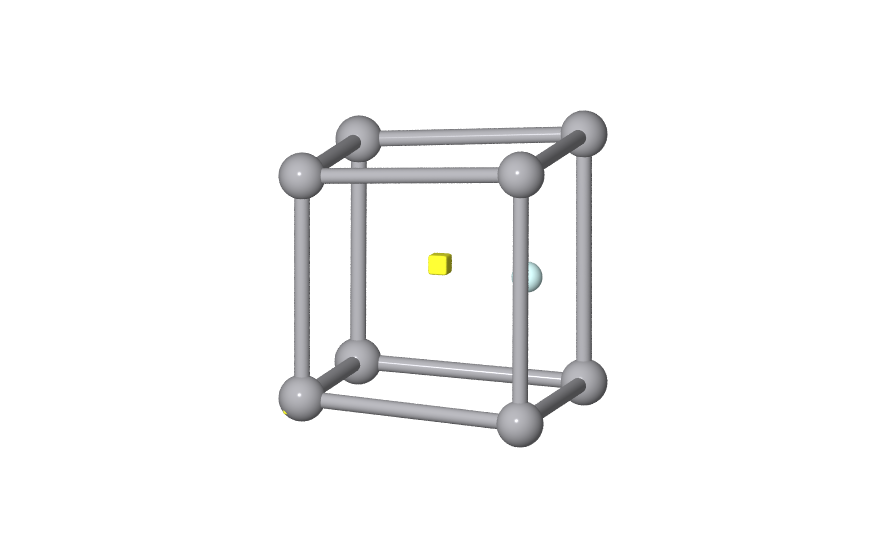
\includegraphics[scale=0.1]{figures/V/v1he_seq/frame14.png} \\
    (a) & (b) & (c) & (d) & (e) \\
 \end{tabular}
 \caption{Migration of He$_1V_1$ cluster in V.
Vacancy, V and He atom are represented with yellow cube, grey and light blue ball respectively.
When the metal atom is placed in the vacancy site the corresponding vacancy cube is not plotted\label{fig:mig:v1he}}
\end{figure}

For this goal, NEB was used in order to search for the minimum energy path of He$V_1$ cluster having in the initial 
and final state of the diffusion process the corresponding lowest energy configurations. 
At first step, the He atom diffuses from initial $O$ site to final 3rd nearest neighbour $O$ site, hopping through
1st nearest $T$ sites (Fig.\ref{fig:mig:v1he} a-d). In a second time, the vacancy migrates along $\langle$111$\rangle$ direction to reach 
its final position corresponding to the initial configuration (Fig.\ref{fig:mig:v1he} e).
This dissociative mechanism has been also experimentally inferred \cite{lewis1988,vassen1991}.
%
The computed DFT migration barrier is about 1.27 eV that correspond roughly to the He-vacancy 
binding energy plus migration barrier of He ($T$ $\rightarrow$ $T$). 
As a result, He increases the diffusion barrier of mono-vacancy by 0.67 eV.

The di-vacancy $V_2^{1nn}$ can migrate into $V_2^{2nn}$ configuration with 0.79 eV barrier. 
Compared to the $V_2^{1nn}$ $\rightarrow $ $V_2^{2nn}$ path, migration from $V_2^{2nn}$ to $V_2^{2nn}$ configuration 
has a lower barrier (0.66 eV). The latter process is a two step mechanism. 

\begin{figure}
 \begin{tabular}{ccccc}
    
\includegraphics[scale=0.1]{figures/V/v2he_seq/frame00.png} &
    
\includegraphics[scale=0.1]{figures/V/v2he_seq/frame02.png} &
    
\includegraphics[scale=0.1]{figures/V/v2he_seq/frame04.png} &
    
\includegraphics[scale=0.1]{figures/V/v2he_seq/frame05.png} &
    
\includegraphics[scale=0.1]{figures/V/v2he_seq/frame06.png} \\
    (a) & (b) & (c) & (d) & (e) \\
 \end{tabular}
 \caption{Migration of He$_1V_2$ cluster in V.
Vacancy, V and He atom are represented with yellow cube, grey and light blue ball respectively.
When the metal atom is placed in the vacancy site the corresponding vacancy cube is not plotted\label{fig:mig:v2he}}
\end{figure}

Firstly, one of the vacancy of the cluster dissociates from the cluster to reach first nearest neighbour site 
in the $\langle 111 \rangle$ direction  changing the geometry of the cluster into a slightly shifted $V_2^{1nn}$ 
configuration (Fig.\ref{fig:mig:v2he} b). Secondly, the second vacancy moves to its nearest neighbour. 
In the same time the He atom goes to its final $O$ position 
between the 2 vacancies where it is in the initial configuration (Fig.\ref{fig:mig:v2he} c-e).  
The trapped He atom roughly doubles the migration barrier of the di-vacancy for both
$V_2^{1nn}$ $\rightarrow $ $V_2^{2nn}$ and $V_2^{2nn}$ $\rightarrow $ $V_2^{2nn}$ paths, 
and increases the barrier by 50$\%$ of the $V_2^{2nn}$ $\rightarrow $ $V_2^{1nn}$ path.

Nevertheless, the presence of He does not change the relative mobility of mono and di-vacancy but moreover, 
it amplifies the gap between mono-vacancy and di-vacancy energy barrier.

\begin{table}
\centering
 \begin{tabular}{c|ccc|ccc}
 \hline
  & \multicolumn{3}{|c|}{V} & \multicolumn{3}{c}{Ta} \\
  \hline
  Configuration & Path & E$^m$ (eV) & Exp. (eV) & Path & E$^m$ (eV) & Exp. (eV) \\
  \hline
  \multicolumn{7}{l}{He interstitial} \\
  \hline
  He & $T$ $\rightarrow$ $T$ & 0.12 & 0.13 \cite{Fedorov1996} & $T$ $\rightarrow$ $T$ & 0.18 &\\
     & $T$ $\rightarrow$ $O$ & 0.26 & & $T$ $\rightarrow$ $O$ & 0.40 &\\
  \hline
  \multicolumn{7}{l}{$V_m$ clusters} \\
  \hline
  Mono-vacancy & 1nn & 0.48 & 0.5 \cite{Fedorov1996} \cite{ullmaier1991} & 1nn & 0.72 & 0.7 \cite{faber1974}\cite{ullmaier1991}\\
   & &  & 0.47 \cite{vanveen1994} & & & \\
  Di-vacancy & 1nn $\rightarrow$ 2nn & 0.34 & & 1nn $\rightarrow$ 2nn & 0.63 &\\
  Di-vacancy & 2nn $\rightarrow$ 1nn & 0.58 & & 2nn $\rightarrow$ 1nn & 0.87 &\\
  Di-vacancy & 2nn $\rightarrow$ 2nn & 0.37 & & 2nn $\rightarrow$ 2nn & 0.55 &\\
  \hline
  \multicolumn{7}{l}{He$_nV_m$ clusters} \\
  \hline
  He$_1V_1$ & 1nn & 1.27 & & 1nn & 1.89 &\\
  He$_1V_2$ & 1nn $\rightarrow$ 2nn & 0.79 & & 1nn $\rightarrow$ 2nn & 1.14 &\\
  He$_1V_2$ & 2nn $\rightarrow$ 1nn & 0.88 & & 2nn $\rightarrow$ 1nn & 1.12 &\\
  He$_1V_2$ & 2nn $\rightarrow$ 2nn & 0.66 & & 2nn $\rightarrow$ 2nn & 1.12 &\\
  \hline
 \end{tabular}
\caption{DFT migration energy barrier, E$^m$ (in eV),  for He, vacancy ($V_m$) and He-vacancy (He$_nV_m$) clusters in V and Ta. The theoretical values of the migration barriers are compared, when is possible, to the corresponding experimental values.  $1nn$ and $2nn$ denote the first and second nearest neighbor configuration of di-vacancy, respectively. 
\label{tab:em}}
\end{table}

\subsubsection*{Tantalum}

The migration barrier of interstitial He in Ta lattice are reported in Tab.\ref{tab:em}. 
The migration barrier of interstitial He are 0.18 eV and 0.40 eV for the $T$ $\rightarrow$ $T$ 
and $T$ $\rightarrow$ $O$ paths, respectively.
The lowest energy migration mechanism correspond to the $T$ $\rightarrow$ $T$, similar to the V case.  

The value of migration barrier of mono-vacancy in Ta is 0.72 eV.
This result is consistent with resistivity annealing experiment which give the value of 0.7 eV~\cite{faber1974}. 
The lowest migration barrier of di-vacancy corresponds to the $V_2^{2nn}$ $\rightarrow$ $V_2^{2nn}$ path. 
Similar to V the last mechanism is more energetically favorable (with 0.55 eV) than the migration of the mono-vacancy.
\wes{These results show a different behaviour compared to Fe \cite{fu2005nat} and W \cite{ODA2014} for which the energy barrier of mono-vacancy and di-vacancy are very close.}

\begin{figure}
 \begin{tabular}{ccccc}
    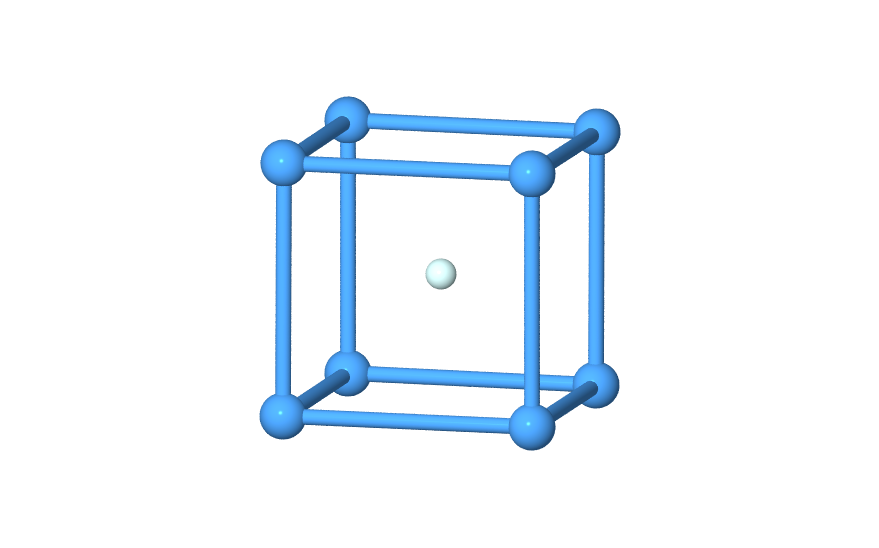
\includegraphics[scale=0.1]{figures/Ta/v1he_seq/frame00.png} &
    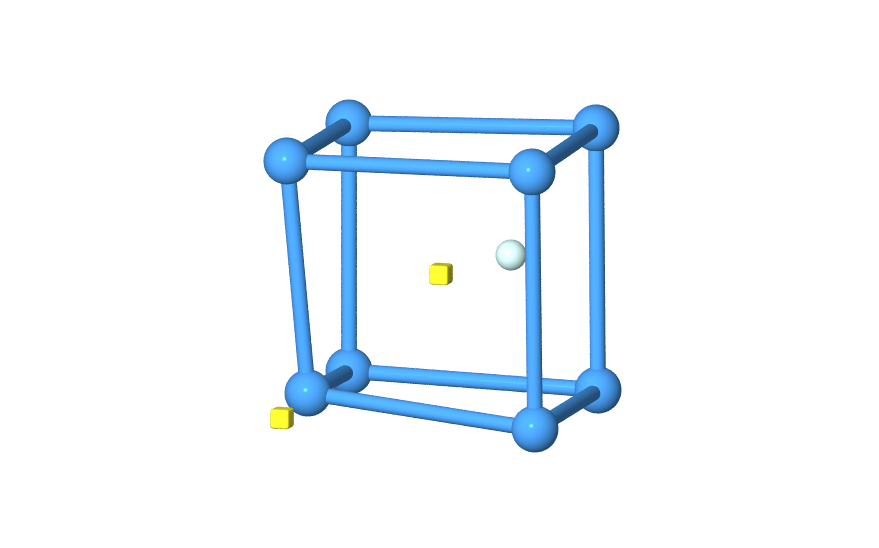
\includegraphics[scale=0.1]{figures/Ta/v1he_seq/frame01.png} &
    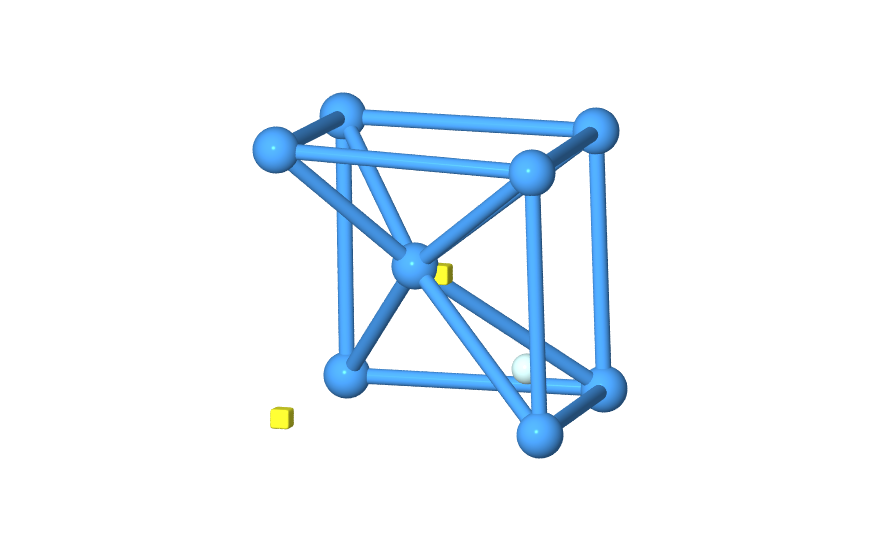
\includegraphics[scale=0.1]{figures/Ta/v1he_seq/frame04.png} &
    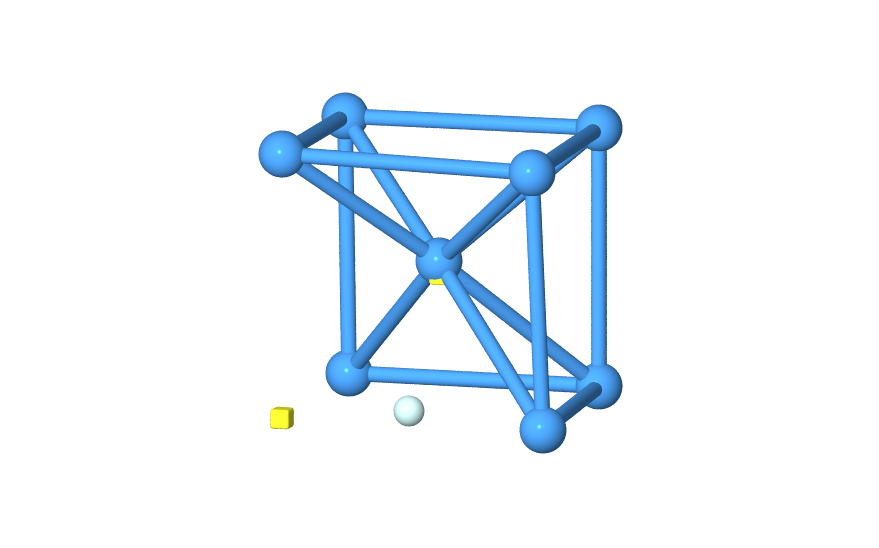
\includegraphics[scale=0.1]{figures/Ta/v1he_seq/frame06.png} &
    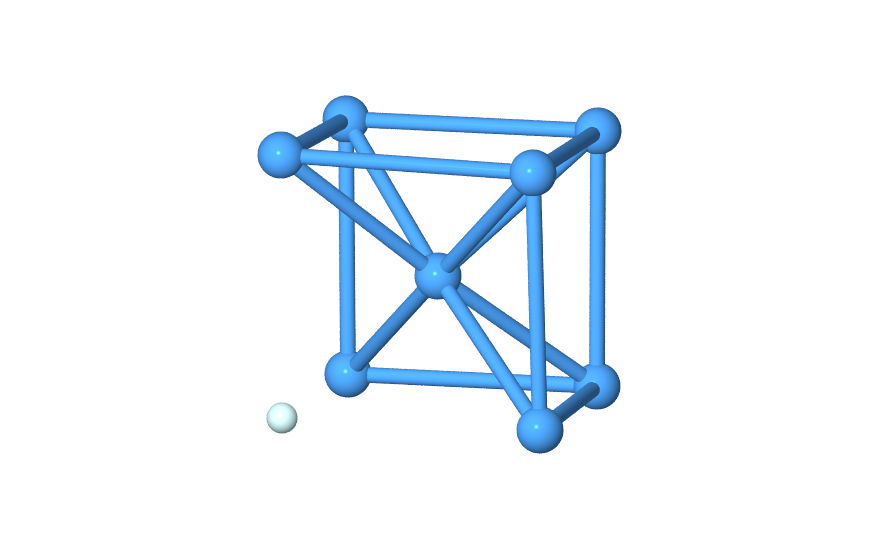
\includegraphics[scale=0.1]{figures/Ta/v1he_seq/frame08.png} \\
    (a) & (b) & (c) & (d) & (e) \\
 \end{tabular}
 \caption{Migration of He$_1V_1$ cluster in Ta.
Vacancy, Ta and He atom are represented with yellow cube, dark blue and light blue ball respectively.
When the metal or He atom is placed in the vacancy site the corresponding vacancy cube is not plotted\label{fig:mig:v1he_Ta}}
\end{figure}

Diffusion of mixed cluster He$_1V_1$ involve firstly  the dissociation of He from the vacancy
to reach the 1st nearest $T$ site (Fig.\ref{fig:mig:v1he_Ta} b). 
Subsequently,  the He atom hops via $T$ interstitial sites while 
at the same time, the vacancy jumps to first nearest neighbour site (Fig.\ref{fig:mig:v1he_Ta} c-d)
Finally, He recombines with the mono-vacancy at $S$ site (Fig.\ref{fig:mig:v1he_Ta} e). This corresponds to the 'impeded interstitial mechanism' or 
'He-vacancy dissociative mechanism' \cite{Trinkaus2003,ullmaier1991} where a He atom diffuses interstitially after it 
dissociates from one vacancy and before being re-trapped by another vacancy.
Diffusion of He$_1V_2$ clusters occurs according to the same scenario described above for V.
The presence of the He atom enhances the migration barrier of mono-vacancy by 1.17 eV.  
For the He$_1V_2$ case, the increase of migration energy due to He is 2 times smaller (0.51 eV) 
for He$_1V_2^{1nn}$ $\rightarrow$  He$_1V_2^{2nn}$ path  than for He$_1V_1$ case.

Contrary to the V case all paths involving He$_1V_2$ clusters have the almost same barrier in presence of He. 
\wes{Consequently, He$_1V_2$ clusters can migrate via these three channels.}
\MCM{Are you sure that are only three ways ? Maybe there are three channels  but did you know the degeneracy of those channels ? Fix that.  }


Thermal desorption spectra experiment give us direct access to dissociation energy we can defined as 
the sum of binding energy and migration energy of He atom or vacancy \cite{Morishita2003}:
\begin{equation}
    E^d_{He/V-He_nV_m} = E^b_{He/V-He_nV_m} + E^m_{He/V}
\end{equation}
In the previous equation, $E_{He/V}$ denotes the corresponding energy related to He or vacancy.
In Fig.\ref{fig:ed} is shown for V and Ta the dissociation energy of He and vacancy with respect to the 
lowest energy configuration of He$_nV_m$ cluster as a function of \textit{n/m} ratio. 
%
This quantity allows to determine whether a mixed cluster tends to emit a He atom or a vacancy to gain stability, 
i.e when E$^d_{He}$ $>$ E$^d_{V}$, the cluster is more likely to dissociate a vacancy.
%
In  Fig.\ref{fig:ed} the crossover between dissociation energy of He or vacancy shows the most stable clusters 
for $\sim$ 0.9 \textit{n/m} ratio with E$^d$ $\sim$ 1.9 eV in V.  
This theoretical result is close to experimental result which indicates E$^d$ = 1.66 eV~\cite{vassen1991},
The corresponding quantities for Ta are estimated to $\sim$ 0.9 \textit{n/m} ratio  and   E$^d$ $\sim$ 2.5 eV.
%
This is consistent with TDS experiment \cite{Fedorov1996} in which the peaks at the highest temperature were attributed 
to the clusters with \textit{n}=\textit{m} for V. 

\begin{figure}
\centering
\begin{tabular}{cc}

\includegraphics[scale=0.35]{figures/V/ratiomax.png}&
% \caption{Dissociation energy of He and vacancy to He$_n$V$_m$ as a function of \textit{n/m} 
% ratio for the most stable clusters in V.
% \label{fig:V_ed}}
% \end{figure}


% \begin{figure}
% \centering
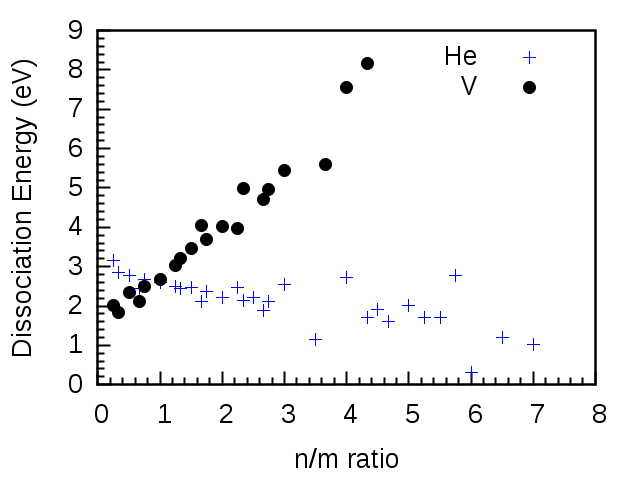
\includegraphics[scale=0.35]{figures/Ta/ratiomax.png}\\
\end{tabular}
\caption{Dissociation energy of He and vacancy from He$_nV_m$ clusters, in V (left panel) and Ta (right panel), as a function of \textit{n/m} ratio. We have taken as reference the configurations with the lowest formation energy.
\label{fig:ed}}
\end{figure}


\section{Conclusion}

We performed first-principle calculations of the formation, binding and migration energy of vacancies 
in the presence or not of He atoms in bcc V and Ta.
In summary, we present our main results :
\begin{itemize}
 \item interstitial He atoms diffuse through tetrahedral sites in both V and Ta.
 
 \item the formation energy of He$_nV_1$ cluster is less than pure interstitial He$_n$ cluster for $n\ge3$ in V 
 and $n\ge2$ in Ta. Consequently, the formation of Frenkel pair is expected when increasing the number of He atom 
 in the interstitial cluster He$_n$.
 
%  Formation of Frenkel pair is expected with growing interstitial He$_n$ clusters 
%  \MCM{growing of interstitial clusterS or interstitial cluster i.e. increasing $n$?. Fix that}, 
%  since the formation energy of He$_nV_1$ cluster is less than pure interstitial He$_n$ cluster for $n\ge3$ in V 
%  and $n\ge2$ in Ta.
% \MCM{be more clear here. You put effect then cause. The natural order is cause and then effect}. 
%  \item In V, He atoms prefer to occupy interstitial sites contrary to Ta case for which He atoms reside 
%  in substitutional sites because of larger density of state \MCM{DOS of what?} at Fermi level for V than for Ta.
 
 \item  for both V and Ta, the formation energy of di-vacancy in $V_2^{2nn}$ configuration  is  lower than 
 the formation energy of $V_2^{1nn}$ configuration. 
 This tendency is also observed in the $VI$ metals such as Mo and W. 
 The di-vacancies in V and Ta have a weak attractive binding energy whereas are repulsive for group $VI$ metals.
 
 \item the effect of He on di-vacancies is to increase the formation energy of the $V_2^{1nn}$ and $V_2^{2nn}$ configurations.
 This increase is more important for $V_2^{2nn}$ than $V_2^{1nn}$ configuration so that the hierarchy is reversed, i.e. 
 $E^f_{He_nV_2^{2nn}} > E^f_{He_nV_2^{1nn}}$ for $n \ge 2$ in V and $n \ge 1$ in Ta. 
 In addition, He atom makes the 1nn configuration more 
 stable than the 2nn configuration. Indeed, the binding energy of He$_{n}V_{2}^{1nn}$ to He atom and mono-vacancy is larger than 
 the binding energy of He$_{n}V_{2}^{2nn}$ to He atom and mono-vacancy when \textit{n} increases.
 
 \item as general tendency  the He atom stabilizes vacancy type clusters and vice versa.
 
 \item \wes{for the 2 studied metals of group $VB$, di-vacancy is more mobile than mono-vacancy. 
 The presence of He atom enhances the migration energy barrier of both mono-vacancy and 
 di-vacancy but also their relative difference.}
 \MCM{I do not understand. If the values are bigger also the differences are. Rewrite}
 
 \item in absence of He, di-vacancy diffuses preferentially via $V_{2}^{2nn}$ $\rightarrow$ $V_{2}^{2nn}$ path 
 in a 2 steps vacancy dissociation-recombination process in both V and Ta.
 
 \item in the presence of He atom, diffusion of both mono-vacancy and di-vacancy involves dissociation of He atom the 
 vacancy type cluster following the 'impeded interstitial mechanism' in both V and Ta case.
 For the di-vacancy diffusion in V, the $V_{2}^{2nn}$ $\rightarrow$ $V_{2}^{2nn}$ path is still favored, but in case of Ta, 
 all paths have the same energy barrier.
 
 \item the most stable clusters have a $n/m$ ratio about 0.9 with a dissociation energy of 1.9 eV and 2.5 eV for V and Ta 
 respectively.
 
\end{itemize}

The present results will be useful as parameters for multi-scale modelling such as kinetic Monte-Carlo simulations or 
cluster dynamics to get insight on the kinetics of the growth of point-defect clusters.

\section*{Acknowledgements}
This work was performed using HPC ressources from the Barcelona Supercomputing Center, CINES and TGCC.
We acknowledge the French Research National Agency (ANR) in the EPIGRAPH project for funding.


\newpage
\bibliographystyle{plain}
\bibliography{article}

\end{document}          
